%% 2/18/2016
%%%%%%%%%%%%%%%%%%%%%%%%%%%%%%%%%%%%%%%%%%%%%%%%%%%%%%%%%%%%%%%%%%%%%%%%%%%%
% AGUJournalSample.tex: this sample file is for articles formatted with LaTeX
%
% This sample file includes commands and instructions
% given in the order necessary to produce a final output that will
% satisfy AGU requirements.
%
% PLEASE DO NOT USE YOUR OWN MACROS
% DO NOT USE \newcommand, \renewcommand, or \def.
%
% FOR FIGURES, DO NOT USE \psfrag or \subfigure.
% DO NOT USE \psfrag or \subfigure commands.
%
%%%%%%%%%%%%%%%%%%%%%%%%%%%%%%%%%%%%%%%%%%%%%%%%%%%%%%%%%%%%%%%%%%%%%%%%%%%%
%
% Step 1: Set the \documentclass
%
% There are two options for article format:
%
% 1) PLEASE USE THE DRAFT OPTION TO SUBMIT YOUR PAPERS.
% The draft option produces double spaced output.
%
% 2) numberline will give you line numbers.

% Tip:
%  To add line numbers to lines in equations:
%  \begin{linenomath*}
%  \begin{equation}
%  \end{equation}
%  \end{linenomath*}

%% To submit your paper:
\documentclass[linenumbers,draft]{agujournal}

% Now, type in the journal name: \journalname{<Journal Name>}
% ie,
\journalname{JGR-Earth Surface}

%% Choose from this list of Journals:
%
% JGR-Atmospheres
% JGR-Biogeosciences
% JGR-Earth Surface
% JGR-Oceans
% JGR-Planets
% JGR-Solid Earth
% JGR-Space Physics
% Global Biochemical Cycles
% Geophysical Research Letters
% Paleoceanography
% Radio Science
% Reviews of Geophysics
% Tectonics
% Space Weather
% Water Resource Research
% Geochemistry, Geophysics, Geosystems
% Journal of Advances in Modeling Earth Systems (JAMES)
% Earth's Future
% Earth and Space Science


%% ------------------------------------------------------------------------ %%
%
%  ENTER Title Page commands:
%
%% ------------------------------------------------------------------------ %%

% (A title should be specific, informative, and brief. Use
% abbreviations only if they are defined in the abstract. Titles that
% start with general terms then specific results are optimized in
% searches)

% Example: \title{This is a test title}

% (List authors by first name or initial followed by last name and
% separated by commas. Use \affil{} to number affiliations, and
% \thanks{} for author notes.
% Additional author notes should be indicated with \thanks{} (for
% example, for current addresses).

% Example: \authors{A. B. Author\affil{1}\thanks{Current address, Antartica}, B. C. Author\affil{2,3}, and D. E.
% Author\affil{3,4}\thanks{Also funded by Monsanto.}}

% (include name and email addresses of the corresponding author.  More
% than one corresponding author is allowed in this LaTeX file and for
% publication; but only one corresponding author is allowed in our
% editorial system.)

%% Corresponding Author:
% Corresponding author mailing address and e-mail address:

% Example: \correspondingauthor{First and Last Name}{email@address.edu}

% Authors are individuals who have significantly contributed to the
% research and preparation of the article. Group authors are allowed, if
% each author in the group is separately identified in an appendix.)

% \affiliation{1}{First Affiliation}
% \affiliation{2}{Second Affiliation}
% \affiliation{3}{Third Affiliation}
% \affiliation{4}{Fourth Affiliation}

%% Keypoints, final entry on title page.
% Example:
% \begin{keypoints}
% \item	List up to three key points (at least one is required)
% \item	Key Points summarize the main points and conclusions of the article
% \item	Each must be 100 characters or less with no special
% characters or punctuation
% \end{keypoints}

%% \begin{abstract} begins second page

%%%%%%%%%%%%%%%%%%%%%%%%%%%%%%%%%%%%%%%%%%%%%%%%%%%%%%%%%%%%%%%%%%%%%
% Track Changes:
% To add words, \added{<word added>}
% To delete words, \deleted{<word deleted>}
% To replace words, \replaced{<word to be replaced>}{<replacement word>}
% To explain why change was made: \explain{<explanation>}

% At the end of the document, use \listofchanges, which will list the
% changes and the page and line number where the change was made.

% When final version, \listofchanges will not produce anything,
% \added{} word will be printed, \deleted{} will take away the word,
% \replaced{}{} will print only the 2nd argument.
% \explain will not print anything.

% Optional argument:
% You can also add additional information to be printed with the list
% of changes, to indicate the initials of the person changing the text,
% and the time and/or date of the change, or any other comment by using
% the optional [] argument:
% \added[AH, 3:30pm, Feb 18, 2016]{added term}
% will yield
% [AH, 3:30pm, Feb 18, 2016] added term on page...
%%%%%%%%%%%%%%%%%%%%%%%%%%%%%%%%%%%%%%%%%%%%%%%%%%%%%%%%%%%%%%%%%%%%%

\begin{document}

%% ------------------------------------------------------------------------ %%
%
%  TITLE
%
%% ------------------------------------------------------------------------ %%

%% REVISION 1
\title{Modeling the Shape and Evolution of Normal-Fault Facets}


%% ------------------------------------------------------------------------ %%
%
%  AUTHORS AND AFFILIATIONS
%
%% ------------------------------------------------------------------------ %%

 \authors{Gregory E.\ Tucker\affil{1},
 Daniel E.\ J.\ Hobley\affil{2}, 
 Scott W.\ McCoy \affil{3},
 and Will T.\ Struble \affil{4}}
 

\affiliation{1}{Cooperative Institute for Research in Environmental Sciences (CIRES) and Department of Geological Sciences,
University of Colorado, Boulder, Colorado, USA.}
\affiliation{2}{School of Earth and Ocean Sciences, Cardiff University, Cardiff, UK.}
\affiliation{3}{Department of Geological Sciences and Engineering, University of Nevada, Reno, NV 89557, USA}
\affiliation{4}{Department of Geosciences, University of Oregon, Eugene, OR, USA}

%% Corresponding Author
%(include name and email addresses of the corresponding author.  More
%than one corresponding author is allowed in this Word file and for
%publication; but only one corresponding author is allowed in our
%editorial system.)

\correspondingauthor{G.\ E.\ Tucker}{gtucker@colorado.edu}

%  List up to three key points (at least one is required)
%  Key Points summarize the main points and conclusions of the article
%  Each must be 100 characters or less with no special characters or punctuation

\begin{keypoints}
\item The longitudinal profiles of facet slopes on extensional footwall blocks exhibit diversity in gradient, shape, and soil cover.
\item
A process-based cellular automaton model with two dimensionless parameters can explain much of the observed variation.
\item  Facet slope angles should record the rate of fault slip on range-bounding normal faults, especially on rocky facets.
\end{keypoints}

%% ------------------------------------------------------------------------ %%
%
%  ABSTRACT
%
%% ------------------------------------------------------------------------ %%


\begin{abstract}
Facets formed along the footwalls of active normal-fault blocks display a variety of longitudinal profile forms, with variations in gradient, shape, degree of soil cover, and presence or absence of a slope break at the fault trace. We show that a two-dimensional, process-oriented cellular automaton model of facet profile evolution can account for the observed morphologic diversity. The model uses two dimensionless parameters to represent fault slip, progressive rock weathering, and downslope colluvial-soil transport driven by gravity and stochastic disturbance events. The parameters represent rock weathering and soil disturbance rates, respectively, scaled by fault slip rate; both can be derived from field-estimated rate coefficients. In the model's transport-limited regime, slope gradient depends on the ratio of disturbance to slip rates, with a maximum that represents the angle of repose for colluvium. In this regime, facet evolution is consistent with nonlinear diffusion models of soil-mantled hillslope evolution. Under the weathering-limited regime, bedrock becomes partly exposed but microtopography helps trap some colluvium even when facet gradient exceeds the threshold angle. Whereas the model predicts a continuous gradient from footwall to colluvial wedge under transport-limited behavior, fully weathering-limited facets tend to develop a slope break between footwall and basal colluvium as a result of reduced transport efficiency on the rocky footwall slope. To the extent that the model provides a reasonable analogy for natural facets, its behavior suggests that facet profile morphology can provide useful constraints on relative potential rates of rock weathering, soil disturbance, and fault slip.
\end{abstract}

%% ------------------------------------------------------------------------ %%
%
%  TEXT
%
%% ------------------------------------------------------------------------ %%



\section{Introduction}
\label{sec:intro}

Mountain fronts in extensional tectonic settings often display facets: steep, basin-facing hillslopes that follow the surface trace of the bounding fault, and mark the transition from footwall to hangingwall (Figure~\ref{fig:facets}). In many cases, dissection of a footwall range by transverse streams creates triangular facets: facet slopes that are flanked by V-shaped transverse valleys, which present a triangular shape when viewed from the adjacent basin (see especially Figures~\ref{fig:facets}a,e,i). In other settings, facets may be trapezoidal in profile, or even compose a more or less continuous surface along a weakly dissected footwall range \citep[e.g.,][]{wallace1978geometry} (Figure~\ref{fig:facets}g,h).

\begin{figure}[ht!]
\centerline{\includegraphics{Figures/facet_photos.pdf}}
\caption{Examples of normal-fault facets. (a) mountain front in Lake Baikal Rift Zone, Russia. (b) Kung Co half graben, Tibet. (c) Hatay Graben, Antakya, Turkey \citep{boulton2009quantifying}. (d) Wasatch fault system, Provo section, near Springville, Utah, USA. (e) west side of Sangre de Cristo range, San Luis Valley, Colorado, USA. (f) Star Valley fault, Wyoming, USA. Note fault trace (light blue dotted line) at base of range front. (g) Magnola fault, central Apennines, Italy. Vegetation break marks approximate location of fault trace. (h) Portion of the Fucino fault near Gioi di Marsi, Italy. Fault trace shown in light blue dotted line. (i) Wasatch fault system, Nephi section, Utah, USA. Fault trace shown in light blue dotted line.}
\label{fig:facets}
\end{figure}

This paper explores the sculpting of facet cross-sectional profiles, using a process-based numerical model as an interpretive tool. We examine the extent to which the model can account for the diversity in facet morphology, and in particular diversity in slope angle, regolith cover, profile shape, and presence or absence of a slope break across the range-bounding fault. We also use the model to frame testable predictions for the relationship between facet morphology, erosion rate, and fault slip rate.



\section{Background}

Fault scarps and facets have intrigued geologists since at least the late 19th century, when mapping expeditions in western North American brought surveyors and geologists to the spectacular terrain of the Basin and Range physiographic providence. Among the first published remarks and illustrations on facet geomorphology in the western USA were those of \citet{gilbert1875report,gilbert1928studies} and \citet{davis1903mountain,davis1909geographical}. Both viewed facets as exhumed fault planes, with only minor modification by erosion. Later workers, however, noted a discrepancy between the dip angle of facets and of the fault planes beneath. Where facets often dip between 20$^\circ$ and 35$^\circ$ \citep{davis1903mountain,davis1909geographical,pack1926new,blackwelder1928recognition,gilluly1928basin,fuller1931geomorphology,anderson1977compound,wallace1978geometry,menges1990soils,petit2009faceted,wilkinson2015slip}, the bedrock fault planes below commonly form angles of 50$^\circ$ to 70$^\circ$ with respect to the horizontal \citep{schneider1925discussion,pack1926new,blackwelder1928recognition,gilluly1928basin,fuller1931geomorphology,wallace1978geometry,wilkinson2015slip}. The difference in dip between a normal fault plane and the facets above it implies that facets, despite their often strikingly planar form, are erosionally modified features \citep{pack1926new,gilluly1928basin}. \citet{gilluly1928basin}, in his work on the Oquirrh Range (Utah, USA), pointed out an interesting implication of this erosional modification: ``as the dip of the fault averages more than 60 degrees along this part of the range front, a wedge having an apical angle of 30 to 40 degrees has evidently been removed from each facet.'' Because the tip of a facet gets exposed to erosion earlier than the base, it undergoes more cumulative erosion. In this sense, the tip of a facet may be considered geomorphically ``older'' than the base \citep{gilbert1928studies,wallace1978geometry,menges1990soils}.

An unusually well-documented example of the contrast between fault plane and facet morphology comes from a study of the Campo Felice fault in the Italian central Apennines by \citet{wilkinson2015slip}. Detailed maps of the Campo Felice fault plane obtained from terrestrial laser scans of the bedrock fault scarp, together with ground-penetrating radar images of the fault plane in the subsurface, revealed a fault dipping at 57$\pm 4^\circ$, whereas the facet surface above the exposed fault plane dips at 40$\pm 5^\circ$ and the debris below the fault trace dips at $36\pm 3^\circ$. Along the Campo Felice, therefore, Gilully's ``removed wedge'' would have an apical angle of about 17$^\circ$.

Facets show a wide diversity in morphology. Although the dip angles of many facets range between 20$^\circ$ and 35$^\circ$, facets have been reported to have dips as low as several degrees \citep[e.g.,][]{menges1990soils,struble2019mountain} or as high as $\ge40^\circ$ \citep[e.g.,][]{wilkinson2015slip,struble2019mountain} (Figure~\ref{fig:profiles1}). Their apices may vary in height from tens to hundreds of meters above the fault trace. Some facets are more or less continuously mantled in soil, as for example those along a portion of the Sangre de Cristo Range in New Mexico, USA studied by \citet{menges1990soils}, as well as on some facets along the eastern margin of the American Basin and Range (Figure~\ref{fig:facets}d,f,i). Others, including facets developed on carbonate rocks in the Italian central Apennines, are rocky, with a shallow, discontinuous colluvium \citep{tucker2011geomorphic} (Figure~\ref{fig:facets}g,h). The longitudinal profiles of facets may be planar, slightly convex-upward, or slightly concave-upward (Figure~\ref{fig:profiles1}). Some faceted mountain fronts display a clear break in slope between the base of the facets and an adjacent colluvial apron (Figure~\ref{fig:facets}g, \ref{fig:profiles2}c,d). For example, facets and adjacent colluvial wedges surveyed by \citet{bubeck2015tectonic} in the Apennines showed a distinct slope break. Along other mountain fronts, the basal colluvium dips at a similar angle to the facet above (Figure~\ref{fig:profiles2}a,b), with the contact between the two sometimes marked by a fault scarp (Figure~\ref{fig:facets}h), and sometimes obscure (Figure~\ref{fig:facets}i).

\begin{figure}[ht!]
\centerline{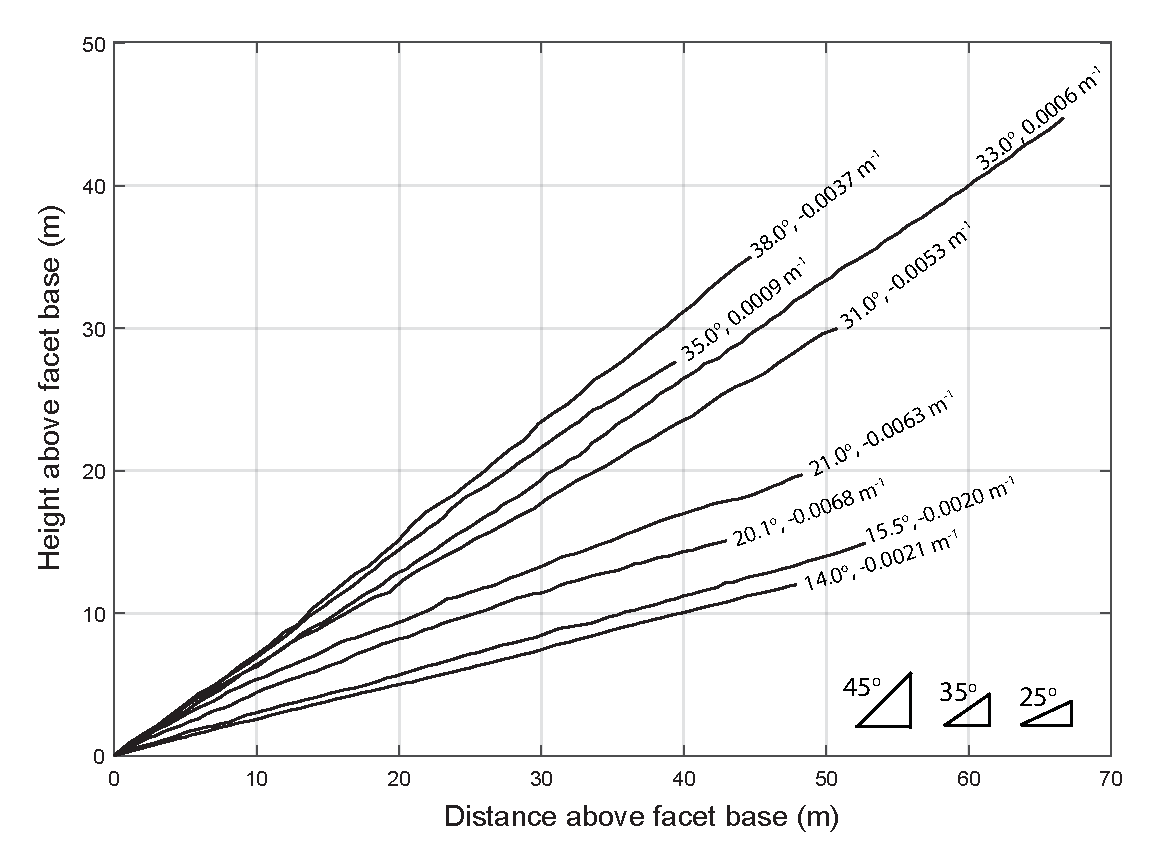
\includegraphics[width=6in]{Figures/FacetShape_bw_trimmed.pdf}}
\caption{Selected facet profiles from four segments of the
Wasatch Fault Zone (Fayette, Levan, Nephi, Brigham City). Profiles
labeled by mean slope angle and concavity. Base of each facet lies just 
above the colluvial wedge and any fault scarp. (Profile coordinates listed in Table S2)}
\label{fig:profiles1}
\end{figure}

\begin{figure}[ht!]
\centerline{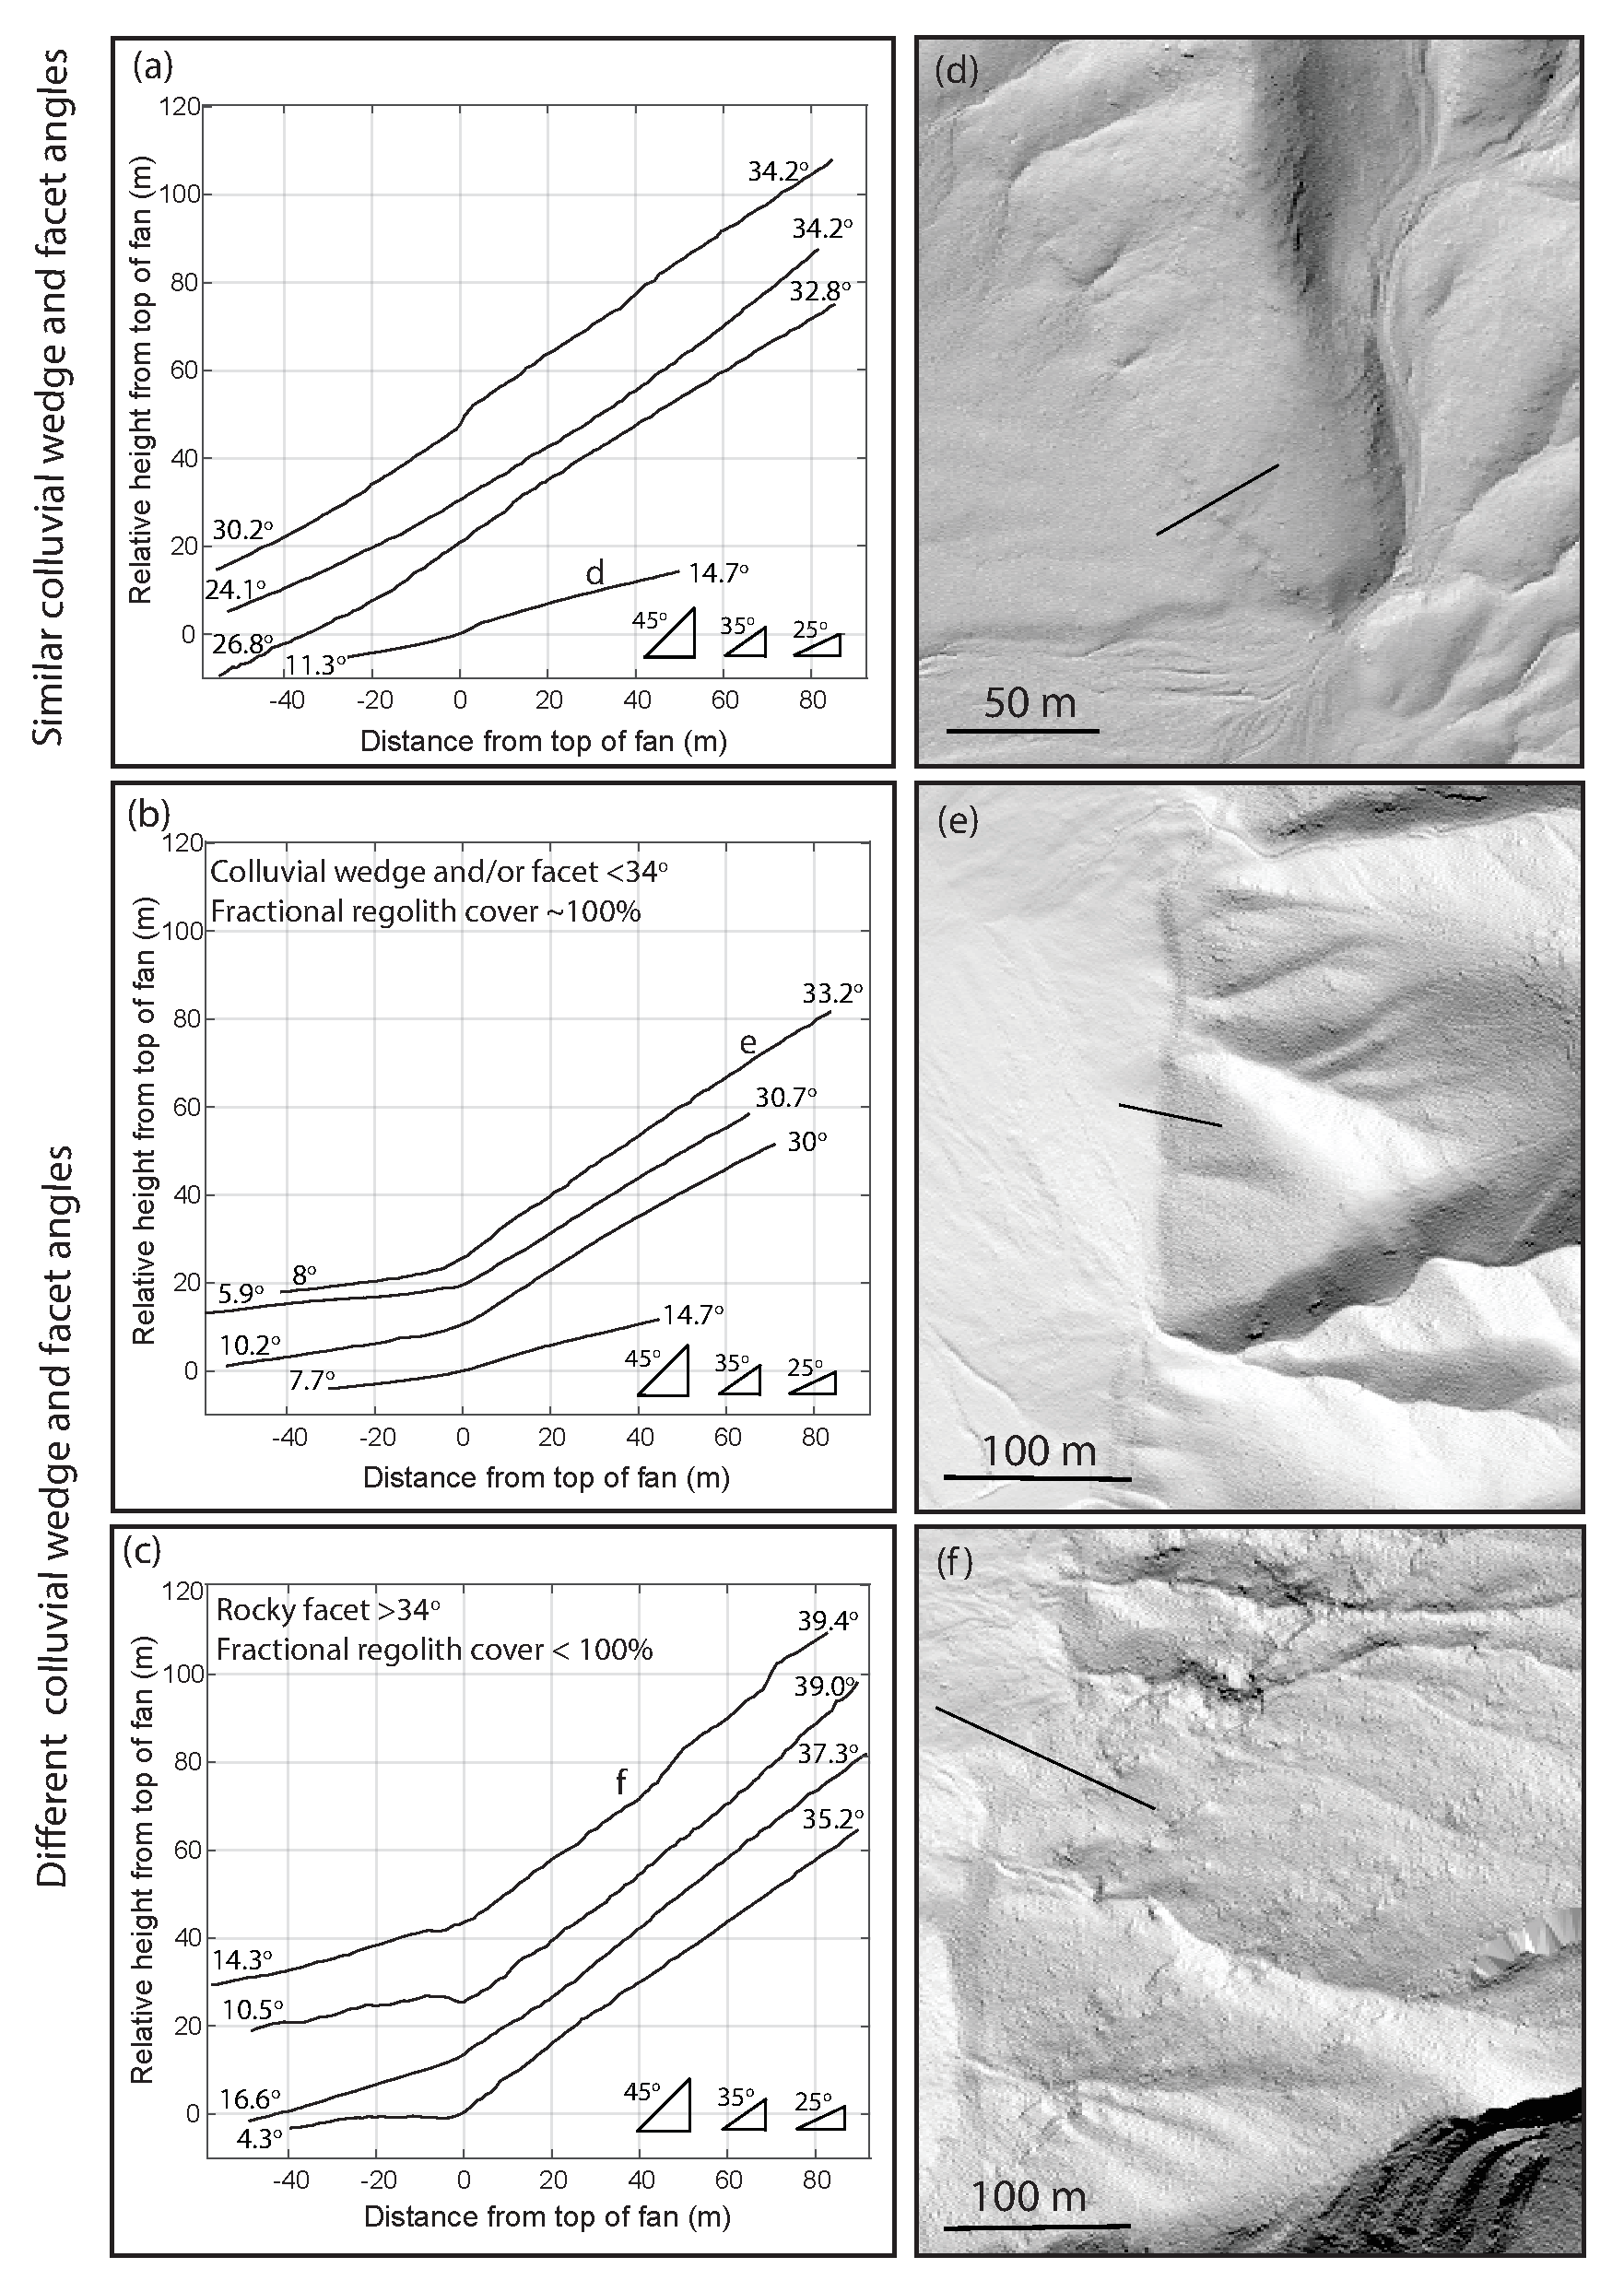
\includegraphics[width=3.9in]{Figures/FacetSlopes4_bw_facetfan_vertical.pdf}}
\caption{Selected facet and colluvial wedge profiles from
three segments of the Wasatch Fault Zone (Fayette, Levan, Nephi). (a)
Facet and colluvial wedge profiles for which the 
facet and colluvial wedge have similar slope angles. (b) Facet and
colluvial wedge profiles for which the slope of both is less than 34$^\circ$, 
and fractional regolith cover nears 100 percent, but where the facet
and colluvial wedge exhibit differt slopes. (c) Facet and colluvial
wedge profiles for which the slope of the facet is greater than 34$^\circ$
and the surface of the facet appears rocky (fractional regolith cover
$\le$100\%). %In (a), (b), and (c), plotted measurements at bottom and top of profiles are slopes of the colluvial wedge and facet, respectively.
(d), (e), and (f) LiDAR hillshade examples of profiles in relation to
topography. (d) Gentle and smooth slopes with uniform regolith cover.
(e) intermediate slope with uniform regolith cover. (f) steep
slope with bedrock exposed. Line segments
correspond to plotted profiles in (a), (b), and (c). Fractional soil
cover estimated from LiDAR hillshade and field observations. (Profile coordinates listed in Table S3)} 
\label{fig:profiles2}
\end{figure}


The diversity in facet morphology raises the question of whether facets may encode useful information about tectonic processes, as several studies have suggested. \citet{hamblin1976patterns} and \citet{anderson1977compound} identified flights of facet-like surfaces along the Wasatch Front (Utah, USA) separated by bench-like spurs, and interpreted these as reflecting alternating episodes of rapid slip and tectonic quiescence. \citet{menges1990soils} noted that facets along the southern Sangre de Cristo Range tend to be steeper and taller toward the middle of fault segments, as opposed to zones of overlap between adjacent segments. \citet{depolo2000estimating} compiled morphologic data on 45 normal faults with independent slip-rate estimates in the arid to semi-arid environment of the Great Basin, USA. Faults with a slip rate in excess of a few tens of microns per year were associated with facets, and among these, \citet{depolo2000estimating} demonstrated a correlation between slip rate and facet height. In a study of facets along four segments of the Wasatch fault system, \citet{zuchiewicz2000geometry} noted multiple potential controls on facet geometry, including lithology, but they considered slip rate to be the primary control. In laboratory experiments by \citet{strak2011interaction}, facet angle increased with slip rate up to a limiting threshold angle. By contrast, \citet{densmore1998landsliding} and \citet{ellis1999development} suggested on the basis of numerical model experiments that facet erosion might be controlled chiefly by bedrock landsliding, such that facet angle represents a threshold angle for stability that does not correlate with slip rate.

If facets take shape through a collaboration between tectonics and erosion, then it stands to reason that their morphology might also encode useful information about rates of geomorphic processes. \citet{menges1990soils} noted, for example, that the degree of soil development generally increases upslope on facets along the southern Sangre de Cristo Range. Using a simple geometric model, \citet{tucker2011geomorphic} noted that the difference in dip angle between a facet and its basal fault---in other words, the apical angle of Gilluly's wedge of missing rock ($\beta$ in Figure~\ref{fig:facetschem})---could be related quantitatively to the ratio of the rates of fault slip and facet erosion. Expressed in terms of surface-normal erosion rate $E_n$ (as opposed to the arc-wise vector used in the original paper), the relation is:
\begin{equation}
\sin \beta = \sin ( \alpha - \theta ) = E_n / V,
\label{eq:predangle}
\end{equation}
where $\alpha$ is the fault dip angle, $\theta$ is the facet dip angle, and $V$ is the fault slip rate. The concept is illustrated in Figure~\ref{fig:facetschem}. One implication of the geometry illustrated in Figure~\ref{fig:facetschem} is that if one knew the fault slip rate and the fault dip, one could estimate the erosion rate (averaged over the age of the facet). Conversely, independent knowledge of the erosion rate would allow estimation of the slip rate.

\begin{figure}[ht!]
\centerline{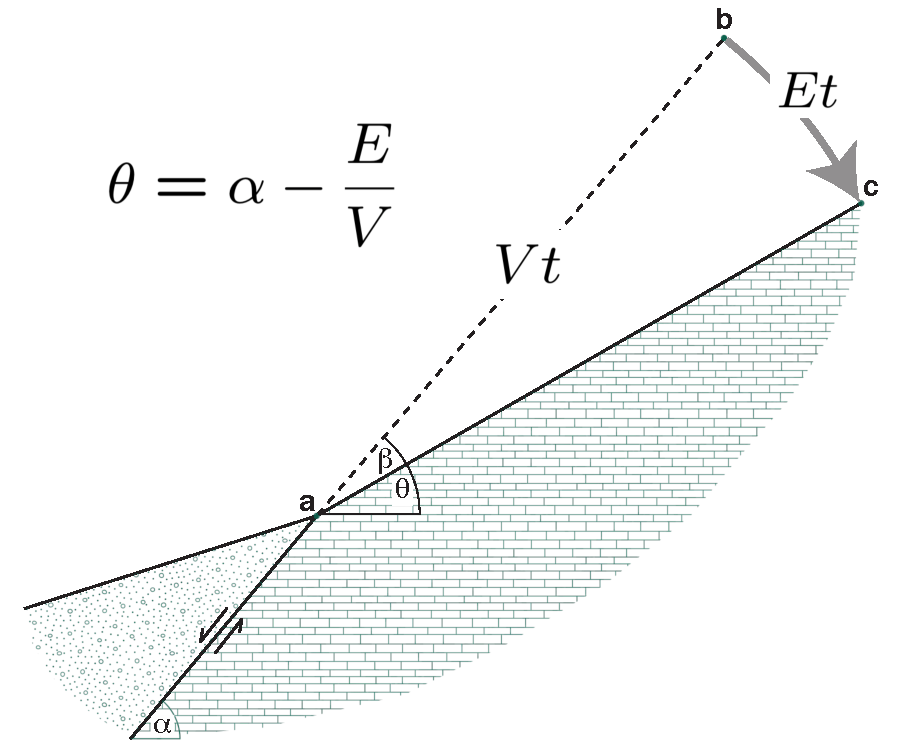
\includegraphics{Figures/facet_schematic.pdf}}
\caption{Conceptual illustration showing how fault slip rate, $V$, fault dip angle, $\alpha$, and slope-normal erosion rate, $E_n$, combine to set the dip angle of a facet profile. $E_v$ is the vertical erosion rate. (Modified from \citet{tucker2011geomorphic}.)} 
\label{fig:facetschem}
\end{figure}

The geometric view of facets as surfaces that erode as they emerge from below ground leads to the question of what factors determine the erosion rate on a normal-fault facet---and this in turn requires us to understand the governing geomorphic processes acting on the surface. \citet{wallace1978geometry} hypothesized that fault scarps created by tectonic offset should relax relatively quickly from the initial fault dip to a more stable angle of 30 to 37$^\circ$, and thereafter lay back much more slowly. As noted earlier, \citet{densmore1998landsliding} and \citet{ellis1999development} proposed, on the basis of numerical model experiments, that many facets form by bedrock landsliding, and that the facet surfaces essentially represent failure planes. \citet{petit2009faceted} questioned this interpretation, in part because of the scarcity of features such as head scarps and debris lobes that one would expect to be associated with bedrock landsliding. Our own observations of facets in the Italian Apennines and the Wasatch fault system, USA, also lead us to support the view of \citet{petit2009faceted} that facets commonly undergo progressive weathering and erosion, as opposed to deep-seated landsliding, though one can identify occasional landslide scars and debris along parts of the Wasatch fault system. \citet{menges1990soils} suggested that facets might be effectively transport-limited, yet the fact that some facets have extensive bedrock outcrops suggests that this is not always the case. Whereas \citet{menges1990soils} noted some evidence for slope wash, \citet{gilbert1928studies} argued that ``rains accomplish little in the way of erosion... [due to] absorption and retardation by porous talus and in conditions unfavorable to concentration of flow.'' Finally, variation in facet morphology and scale with lithology implies that facet materials differ in their susceptibility to weathering and transport \citep{menges1990soils,zuchiewicz2000geometry}. 

Numerical models of extensional mountain range evolution can reproduce classic landforms such as facets, spurs, and wineglass-shaped valleys (wide in the headwaters and narrowing downstream; e.g., \citep{leeder1993interaction}), but models differ in their representation of the governing processes. \citet{densmore1998landsliding} and \citet{ellis1999development} introduced a model that included rock weathering, regolith creep, and bedrock landsliding, and explored a part of the parameter space in which facet erosion occurred primarily by landsliding. A model developed by \citet{petit2009faceted} represented hillslope erosion using a diffusion formulation, with a higher transport coefficient applied to slopes steeper than $40^\circ$. In their study of facets in the Great Basin, \citet{depolo2000estimating} showed that the observed relationship between slip rate and facet angle was consistent with a nonlinear diffusion model. Similarly, analysis of facets along the Wasatch fault system by \citet{struble2019mountain} suggested a nonlinear relationship between erosion rate and facet angle. The planform landscape evolution model studied by \citet{petit2009faceted} showed little correlation between facet slope and fault dip angle, whereas the geometrical analysis of \citet{tucker2011geomorphic} implies that fault dip should be a primary control. In summary, the community has developed several published models of landscape evolution on extensional footwalls, but the implications of these models for facet evolution differ depending on the assumed process rules. To make further progress, we need models that can account for the observed diversity in facet morphology, including variations in slope angle, regolith cover, and shape, and that make field-testable predictions about the relationship between morphology, erosion rate, and slip rate.


\section{Approach and Scope}

We view normal-fault facets as unique natural experiments: slopes that are born as steep, seismo-tectonic fault scarps, and undergo progressive weathering and erosion as they are translated upward and away from the fault trace. We use a process-oriented cellular automaton model of facet cross-section evolution as an interpretive tool with which to address the following questions: can a model that combines rock weathering with disturbance-driven soil creep account for the observed range in facet angle, regolith cover fraction, shape, and colluvial wedge angle? If so, what are the primary controlling factors? Does the model imply a systematic relationship between facet angle, erosion rate, and fault slip rate, and if so what does that relationship look like? The answer to this last question is especially important, because it sets up a testable prediction: facet angle is easy to measure, and erosion rate can in principle be obtained either through the geometric method summarized in Figure~\ref{fig:facetschem} (if fault slip rate is known), or by techniques such as cosmogenic nuclide analysis.

We focus on the cross-sectional geometry of facets, rather than their full three-dimensional (3D) form; in other words, our interest is not in explaining why facets are often triangular (which simply reflects the geometry of transverse canyons), but rather in understanding what sets their gradient, profile shape, and regolith cover. That said, the influence of facet length---the distance between the fault trace and the facet's upper edge at a particular cross-sectional position---is considered by comparing models with varying domain length, as described below. We do not consider controls on the height of the facet edge, as this clearly depends in part on the spacing between transverse channels, and on the topography of valley side slopes along them. We further restrict our consideration to unchanneled facet surfaces, where incision by concentrated flow plays little or no role. Finally, our main focus is on normal-fault facets, rather than facet-like features that  form by other means, such as folding or rapid river incision \citep[e.g.,][]{cotton1950tectonic}, though there are obvious similarities. Steep slopes formed by rapid vertical baselevel fall have been studied theoretically using a version of the same model that we apply here \citet{tucker2018lattice}.

Note that we use the terms ``soil,'' ``regolith,'' and ``colluvium'' interchangeably to refer to loose granular material on a hillslope. We do not distinguish among the properties of different types of soil or other granular material, but instead consider the primary material contrast to be the different between bedrock, and the disaggregated, granular material that results when that rock has been sufficiently weathered.

%A cellular automaton might seem like an odd choice for modeling the evolution of an idealized hillslope cross section. After all, most models of hillslope cross-sectional morphology are built on differential equations, which are sometimes viewed as ``the keys to geomorphic nirvana'' \citep{bras2003six}. In this case, however, it is the only model we know of that 

\section{Cellular Hillslope Evolution Model}

We model facet profile evolution using a continuous-time stochastic cellular automaton method. With this method, the spatial domain is represented using a discrete lattice of cells, while the dynamics are modeled by cell-state transition events that occur at random intervals in time, according to specified rate coefficients \citep{narteau2001small,narteau2009setting}. This approach offers several important advantages for modeling facet slope evolution. First, it accounts for a continuous range of slope forms, from smooth, soil-mantled slopes, to steep, irregular, and rocky ones \citep{tucker2018lattice}. It provides a direct treatment of stochastic disturbances, rather than lumping their effects into a ``black-box'' rate coefficient, and these disturbances can trigger both short-range and long-range (nonlocal) sediment motion, depending on topography. Nonetheless, the model's parameters can be translated to rate coefficients for weathering  and sediment transport \citep{tucker2018lattice}. Furthermore, because the cellular framework allows a fully two-dimensional representation (as opposed to the more common profile representation, in which surface elevation is a function of one independent spatial dimension), it provides a natural way to treat combined vertical and horizontal tectonic offset. Finally, the cellular approach described below (and in greater detail by \citet{tucker2016celllab,tucker2018lattice}) honors the occurrence of a patchy or otherwise incomplete regolith cover, as is observed on some facet surfaces.

The facet profile evolution model builds on the ``Grain Hill'' cellular automaton framework \citep{tucker2018lattice}, with the addition of a 60$^\circ$ dipping normal fault. The model domain consists of a lattice of hexagonal cells that represents a vertical cross-section through a hypothetical facet and its adjacent colluvial wedge (Figure~\ref{fig:domainschematic}). The height of each hexagonal cell (defined as twice the apothem, which is the distance from hexagon's center to the midpoint of one of the sides) is denoted by $\delta$. The lower left corner of the model represents a longitudinal stream that removes any debris delivered to it, and whose elevation can either be fixed to the hangingwall block or allowed to rise over time at a prescribed rate. In either case, the hangingwall serves as the reference frame for the model. The right side of the model represents the upper edge of the facet at that particular cross-section; increasing or decreasing the width of the domain broadly equates to moving the cross section toward or away from the facet tip (Figure~\ref{fig:domainschematic}).

\begin{figure}[ht!]
\centerline{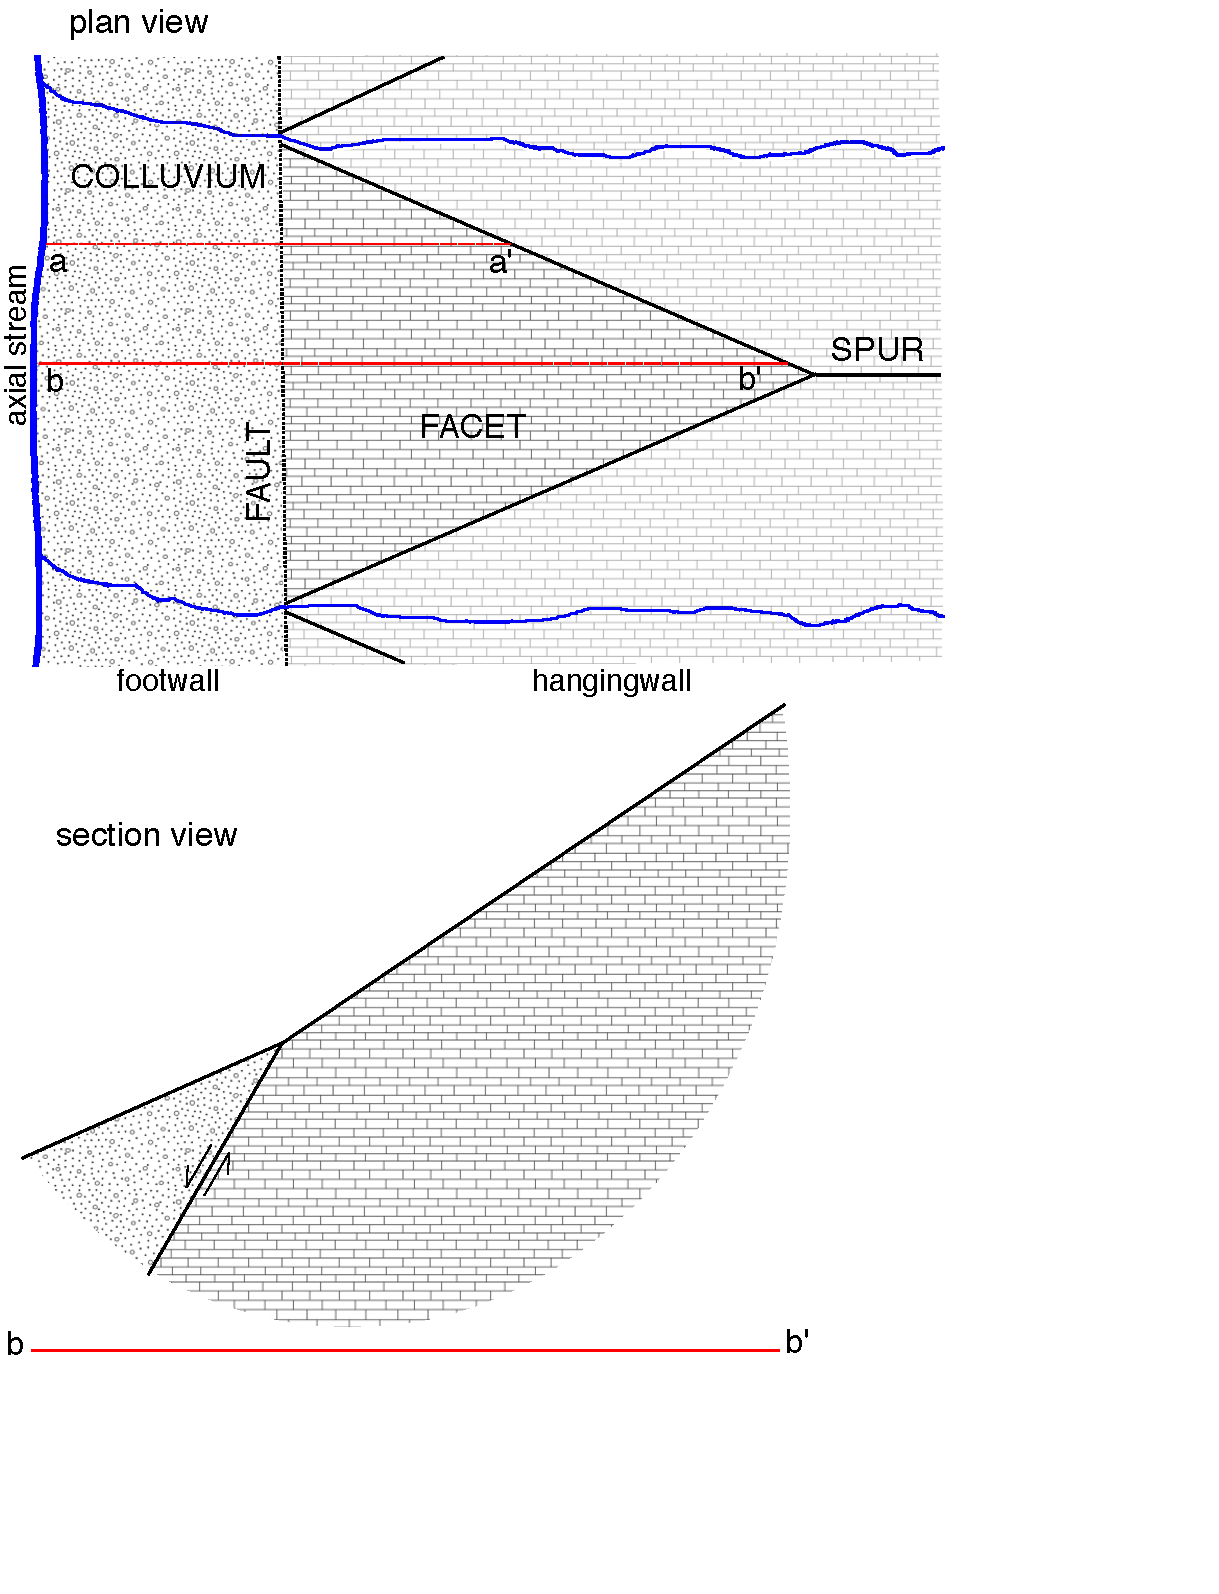
\includegraphics[scale=0.6]{Figures/facet_plan_and_profile.pdf}}
\caption{Schematic illustration of model domain, which represents a vertical cross-section through an idealized facet and its adjacent colluvial wedge. Right side of domain represents the upper edge of facet, and left side represents a longitudinal stream in the hangingwall that removes any debris delivered to it. Changing the position of the cross section (for example, from a--a' to b--b'), and therefore its length, is accomplished by changing the width of the model domain.}
\label{fig:domainschematic}
\end{figure}

Each hexagonal model cell represents one of three types of material: air, rock, or regolith (Figure~\ref{fig:cellstates}). Regolith cells may be stationary, or may be in a state of motion in one of the six lattice directions. Collectively, these materials and motion directions are represented by assigning one of nine integer state codes to each cell in the domain (one each for air, rock, and stationary sediment, plus one for each of the six motion directions). Stochastic, pairwise transitions represent the processes of rock weathering, regolith disturbance, and ensuing regolith motion \citep{tucker2016celllab,tucker2018lattice}. For example, the rock cell in a rock-air pair has a user-specified probability per unit time of transitioning to a regolith cell, representing weathering. Instead of clicking through a series of time steps of fixed duration, the model iterates over a sequence of these stochastic-in-time transition events, in which one or both cells in an adjacent pair change state. The algorithm works by scheduling each potential transition event at a randomly generated future time, using an exponential probability distribution function of inter-event waiting times. The program then iterates in chronological order through these scheduled events. As the domain evolves, new transitions are scheduled, and some previously scheduled ones are invalidated. \citet{tucker2016celllab} provide a comprehensive description of the continuous-time stochastic framework and the algorithms that implement it.

\begin{figure}[ht!]
\centerline{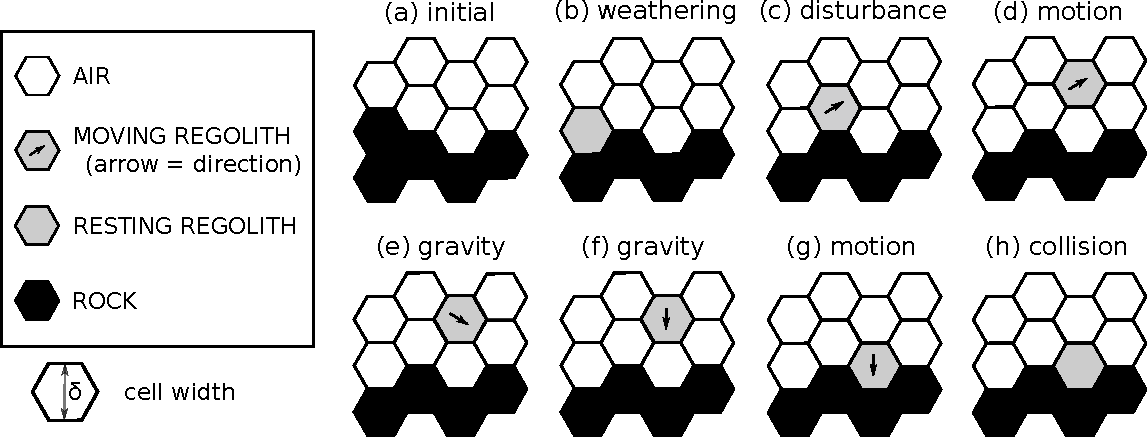
\includegraphics[scale=0.7]{Figures/cell_states_and_transitions.pdf}}
\caption{Illustration of cell states and pairwise transitions in the Grain Facet model, with examples of several transitions. Each cell assigned an integer from 0 to 8 that represents its state (0 is fluid, states 1--6 represent the six directions of motion, state 7 is stationary regolith, and state 8 is rock). (Figure modified from \citet{tucker2018lattice}).}
\label{fig:cellstates}
\end{figure}

\citet{tucker2018lattice} present the rule set for the Grain Hill model. Here, we briefly summarize these rules, and describe two additions to the original version: the implementation of periodic slip on a $60^\circ$ dipping normal-fault, and the addition of a rule that represents dissolution of bedrock. Adding the dissolution rule permits comparison of the numerical model with a simple analytical expression, and also acknowledges the occurrence of facets in soluble rock, such as the platform carbonates common to the Mediterranean region.

To represent normal-fault slip, a $60^\circ$-dipping fault crosses the grid lattice at a user-specified location (Figure~\ref{fig:domainschematic}, bottom). Fault slip is treated as quasi-steady, with small slip events occurring at regular intervals. During each slip event, cells in the footwall block are shifted up and to the right on a 60$^\circ$ angle, with a displacement distance of $\sqrt{3}$ lattice units per time interval $\tau_s$. We will also make use of a related quantity, $\tau= \tau_s / \sqrt{3}$, which is the average time interval between unit slip events. The slip rate is therefore $V = \delta / \tau$ [L/T], where $\delta$ is the width of a grid cell; slip rate is controlled in the model by setting $\tau$. Note that the square brackets here and below are used to indicate the dimensions of certain quantities, with L denoting length and T denoting time (so for example ``[L/T]'' should be read as ``this variable has units that represent length per time,'' such as meters per second, fathoms per fortnight, or potrzebies per kovac \citep{knuth1955potrzebie}). 

Production of regolith from bedrock is represented by a transition from a rock-air pair to a regolith-air pair (Figure~\ref{fig:cellstates}, a to b). The rate constant $w$ [1/T] represents the average transition frequency. We denote the corresponding characteristic weathering velocity as $W=\delta w$ [L/T]. Given a cell width of $\delta$, the expected bare-bedrock weathering rate is $2a W$, where $a$ is a surface-roughness coefficient (described below); the factor of two reflects the fact that for a planar surface, the hex lattice geometry exposes an average of two faces per cell. Note that the model's treatment of weathering means that it effectively occurs normal to the air-rock interface, whatever the orientation of that interface may be.

In order to explore the case of completely weathering-limited slopes, we introduce a second weathering rule to represent dissolution. When this rule is invoked, rock-air cell pairs transition to air-air pairs---representing rock dissolution---with an average rate $s$ [1/T], and a charateristic dissolution velocity $W_s = \delta s$. The expected bare rock dissolution rate [L/T] is therefore $2 a W_s$.

We assume that regolith transport can occur by two means: (1) displacement by a disturbance event and subsequent motion, or (2) spontaneous gravitational failure, when the local angle of repose is exceeded. The model's disturbance rule represents the action of processes like animal burrowing, frost heave, tree throw, and other mechanisms that tend to displace regolith outward from the surface. The disturbance transition rule applies to locations where a resting regolith cell lies adjacent to an air cell. When the transition occurs, the regolith and air trade places, and the regolith state switches from resting to moving in the direction from which disturbance originated (Figure~\ref{fig:cellstates}, b to c). The disturbance rate parameter $d$ [1/T] represents the average disturbance frequency, and functionally equates to the disturbance frequency parameter $N_a$ in the probabilistic theory of soil creep developed by \citet{furbish2009statistical}. The corresponding characteristic disturbance velocity is denoted by $D=\delta d$.  \citet{tucker2018lattice} show that for relatively gentle slopes, the disturbance rate relates directly to the commonly used soil transport efficiency factor (``hillslope diffusivity''), $D_s$, according to
\begin{equation}
d = \frac{D_s}{60 \delta^2}.
\end{equation}
For regolith-mantled slopes steeper than about 15$^\circ$, the effective transport efficiency increases progressively with slope angle, diverging at a 30$^\circ$ effective angle of repose \citep[][their Figure 10]{tucker2018lattice}.

Moving particles follow a set of transition rules that mimic the kinematics of inelastic grain motion in a gravitational field. Although these motion and collision rules are necessarily heuristic, they effectively capture the settling motion of disturbed particles \citep{furbish2009statistical}. The motion, gravitational, and inelastic collision rules are illustrated in Figure~\ref{fig:cellstates}, and described in greater detail by \citet{tucker2016celllab} and \citet{tucker2018lattice}. One rule to note in particular: a regolith cell that lies above and adjacent to an air cell can transition to a moving state, with a high transition rate parameter. Because of the lattice geometry, this rule imposes an effective 30$^\circ$ angle of repose. Regolith cells on slopes steeper than than this will tend to undergo spontaneous downslope motion without requiring a disturbance event to mobilize them. This treatment provides a way to represent ravel transport.

Sensitivity experiments indicate that the exact nature of the motion and settling rules is not especially important (see Supplemental Information). What matters more is that there exists a time-scale separation between disturbance (with intervals on the order of years) and settling (time scale on the order of seconds or less). The rule set described above can capture a range of slope forms, including regolith-mantled and convex-upward forms, planar angle-of-repose, and partially mantled ``rocky'' slopes \citep{tucker2018lattice}. This generality makes the model an appropriate one for exploring bedrock fault scarps and facets, which emerge during earthquakes as steep, rock slopes, and can subsequently evolve into partially or fully regolith mantled erosional slopes. In the following section, we present %model experiments that address three related questions:
%\begin{enumerate}
%\item What conditions are both necessary and sufficient to produce planar facet profiles with a thin  mantle (continuous or discontinuous) of regolith?
%\item Can the model account for the observed range in facet slope angle, cross-sectional shape, soil cover, and facet-to-colluvial-wedge transition?
%\item What is the predicted relationship between facet gradient and erosion rate?
%\end{enumerate}
%We explore these questions with a 
a systematic parameter exploration, beginning with the simple case of a purely weathering-limited slope.


\section{Results}

\subsection{Weathering Limited Case: Facet Dissolution}

We start with a simple test: if a facet erodes at a steady, uniform rate, its evolution should follow the geometry illustrated in Figure~\ref{fig:facetschem}. The profile should be linear, and the dip angle should relate to the rates of erosion and slip according to equation~(\ref{eq:predangle}). To perform this test, we run the model with dissolution activated, and without any rock-to-regolith conversion. On a planar surface, with an average of two faces per cell, the expected average rate of erosion by dissolution would be $2\delta s$. Surface roughness further increases the effective dissolution rate by a factor $a\approx 1.8$ (Supplemental Information, Section S2).

We define a dimensionless dissolution efficiency as the ratio of expected dissolution rate ($2a\delta s$) to fault slip rate:
\begin{equation}
S' = \frac{2a\delta s}{V}.
\label{eq:nddissefficiency}
\end{equation}
Here $2a\delta s$ [L/T] is the expected slope-normal erosion rate, and $S'$ therefore represents the ratio of slope-normal erosion rate to fault slip rate. From equation~(\ref{eq:predangle}), the predicted facet dip angle is
\begin{equation}
\theta = \alpha - \sin^{-1} S',
\label{eq:dissangle}
\end{equation}
where $\theta$ and $\alpha$ are both in radians. Figure~\ref{fig:dissruns} presents simulated profiles for facets eroded by dissolution, under different values of dimensionless weathering rate $S'$. The figure also compares shorter and longer facets (top and bottom rows, respectively). The simulated facets show a linear relation between angle and dissolution rate, consistent with the analytical expectation (equation~\ref{eq:dissangle}) (Figure~\ref{fig:angdiss}). As expected, there is no apparent relation between slope angle and the width of the cross section.

\begin{figure}[ht!]
\centerline{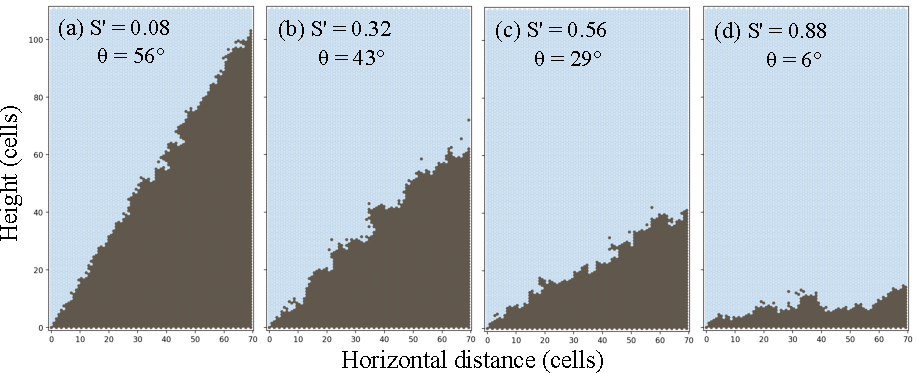
\includegraphics{Figures/dissolution_model_profiles.pdf}}
\caption{Simulated facet cross-sectional profiles formed under a combination of fault slip and dissolution. Dark gray indicates rock, and light blue is air. Labels show the dimensionless effective dissolution efficiency, $S'$ (equation~\ref{eq:nddissefficiency}), and the predicted and simulated average facet slope angle, $\theta$. Line shows facet profile predicted by equation (\ref{eq:dissangle}). Top and bottom rows compare shorter and longer facets.}
\label{fig:dissruns}
\end{figure}

\begin{figure}[ht!]
\centerline{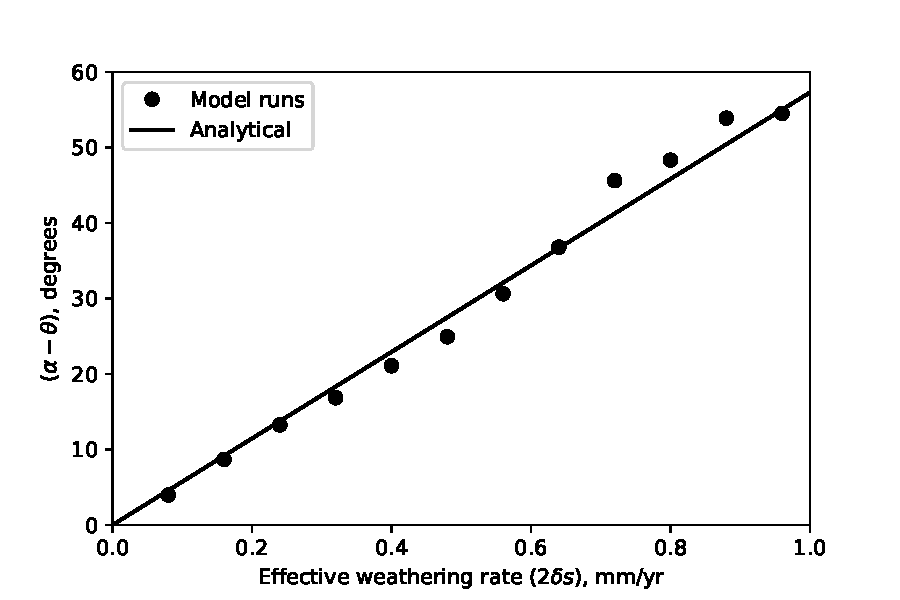
\includegraphics{Figures/angle_vs_dissolution.pdf}}
\caption{Difference in angle between fault plane ($\alpha$) and facet ($\theta$), as a function of the dimensionless dissolution rate $S'$, which is expected dissolution rate divided by the fault slip rate, from runs with fault slip and dissolution (only). Open circles and pluses show individual model runs with shorter and longer facets, respectively (Figure~\ref{fig:dissruns}). Line shows the prediction of equation~\ref{eq:dissangle}. Panels (e) and (f) show runs with the same $S'$ as (a) and (c), respectively, but with longer facets (represented by a wider model domain).}
\label{fig:angdiss}
\end{figure}

\subsection{Facets with Regolith}

We next consider the case in which rock weathers iso-volumetrically to regolith rather than dissolving, with regolith motion driven by stochastic disturbance events (Figure~\ref{fig:cellstates}). Two dimensionless parameters determine the model's behavior:
\begin{eqnarray*}
\textrm{Dimensionless weathering rate:} & w' = W/V = W\tau/\delta = w\tau \\
\textrm{Dimensionless disturbance rate:} & d' = D/V = D\tau/\delta = d\tau.
\end{eqnarray*}
The first of these represents the characteristic weathering velocity ($W$) relative to fault slip rate ($V$), whereas the second represents characteristic disturbance velocity ($D$) relative to fault slip rate.

Figures~\ref{fig:dwprofiles} and \ref{fig:angw} illustrate the role of these two parameters for the case of a facet of fixed length. The model shows three behavior regimes. When $w'\gg d'$, gradient depends on the disturbance frequency regardless of weathering rate. In this transport-limited regime, solutions with $d'\le 1$ produce angle-of-repose slopes (recall that the model has a 30$^\circ$ effective angle of repose) (Figure~\ref{fig:dwprofiles}, panels in upper left quadrant). Although these angle-of-repose solutions are not inevitable, they occupy a large part of the model's parameter space and could be thought of as an attractor state. When $w' < 1$, slope angle depends primarily on $w'$. But even in this weathering-controlled regime, disturbance rate continues to have some influence, except in the extreme dissolution-limited case when there is no regolith to move (Figure~\ref{fig:angw}, solid curve and circles). 

Facet shape depends on both $w'$ and $d'$. With sufficiently effective weathering and transport, represented by the parameter space $w'>1$ and $d'>1$, the model produces convex-upward facets (Figure~\ref{fig:dwprofiles}, upper right). If either of these parameters is less than unity, the model generates planar or nearly planar facets. The regolith cover that forms on these surfaces remains relatively thin (one to a few $\delta$ thick) because the nearly complete cover shields the bedrock from further weathering.

Facet length has little influence on slope angle (compare Figure~\ref{fig:angw} left and right), except in the case of $d'\gg 1$ (star and triangle symbols in Figure~\ref{fig:angw}). Here, longer slopes are systematically steeper, because in this transport-limited, sub-threshold mode, increased downslope regolith flux necessitates a steeper gradient.

\begin{figure}[ht!]
\centerline{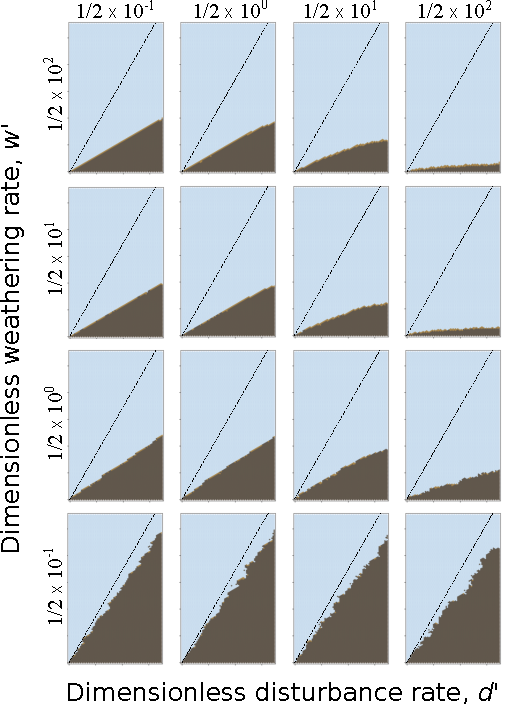
\includegraphics[scale=1.5]{Figures/four_by_four_profiles_in_d-w_space.pdf}}
\caption{Examples of simulated facet profiles at varying values of $d'$ and $w'$. Dotted line shows projected fault plane. Model grids have 111 rows and 81 columns.}
\label{fig:dwprofiles}
\end{figure}

\begin{figure}[ht!]
\centerline{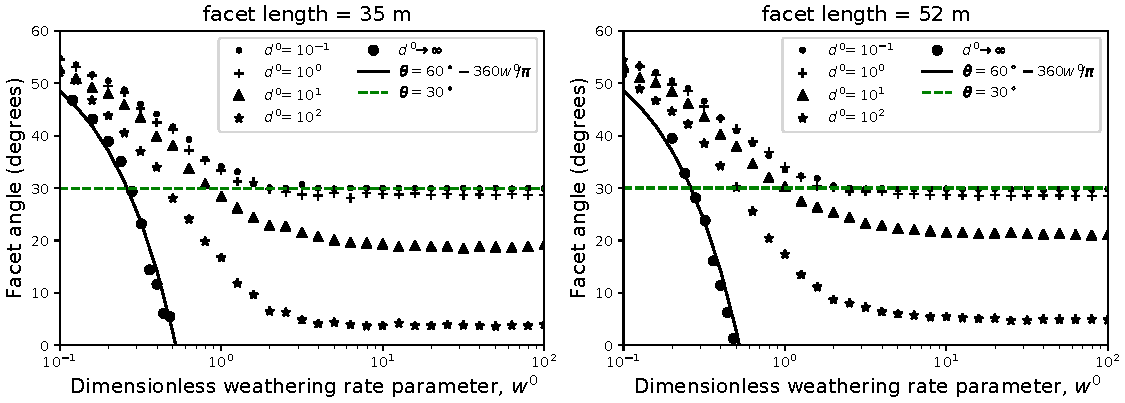
\includegraphics[scale=0.8]{Figures/facet_angle_vs_dw.pdf}}
\caption{Modeled equilibrium facet angle as a function of weathering and disturbance rate parameters. Solid line shows the analytical solution for the case in which no regolith is produced (all rock dissolves), which corresponds to an effectively infinite disturbance rate. Dashed line shows the model's 30$^\circ$ effective angle of repose.}
\label{fig:angw}
\end{figure}

The fractional regolith cover depends mainly on $w'$, and secondarily on $d'$ (Figure~\ref{fig:regw}). The relation follows a sigmoid-like curve, with the steepest segment of the curve corresponding to $w'\approx 1$ and a fractional cover of approximately 50\%. The calculations show $>$80\% cover when $w'>10$, and less than 50\% cover when $w'<1$. For a given $w'$, a facet with a higher disturbance rate will tend have a thinner cover, all else equal. Values of $d'\ll1$ are associated with significantly enhanced stochastic variability in cover percentage in both space and time.

\begin{figure}[ht!]
\centerline{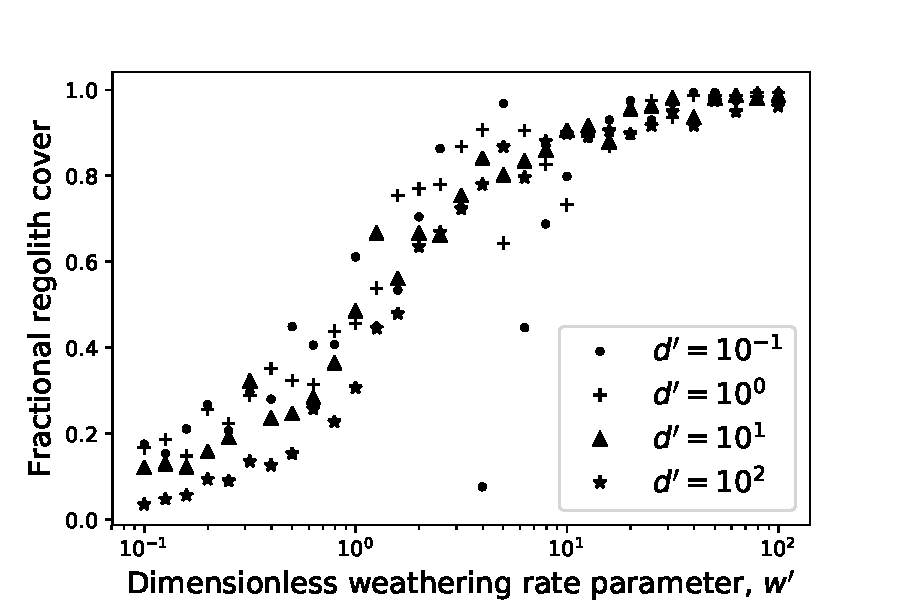
\includegraphics{Figures/reg_cover_vs_wprime.pdf}}
\caption{Modeled regolith cover proportion for facets in quasi-steady state, as a function of weathering and disturbance rate parameters. Scatter around the sigmoidal curve reflects stochastic variability (each data point represents one snapshot in time rather than a temporal average).}
\label{fig:regw}
\end{figure}


\subsection{Colluvial Wedges}

We explore the formation of colluvial wedges with a series of model runs similar to those in Figure~\ref{fig:dwprofiles} but with the fault location shifted to the right (Figure~\ref{fig:colluv}). This geometry places the baselevel outboard of the fault trace, thereby allowing the creation of a colluvial wedge between the fault and baselevel. In the angle-of-repose regime, with $w'>1$ and $d'\le 1$, the wedge shares the same slope gradient as the facet itself, so that the fault trace appears partway up the facet slope (Figure~\ref{fig:colluv}, upper left). Solutions with $w'<1$ and $d'<1$ generate slope breaks because the bedrock facet rises more steeply than the colluvial wedge, which can be no steeper than the angle of repose (Figure~\ref{fig:colluv}, lower left). With $w'<1$ and $d' > 1$, sediment transport becomes efficient enough that the wedge slope is less than the angle of repose  (Figure~\ref{fig:colluv}, lower right). Solutions with $w' \approx 1$ and $d'>1$ produce a relatively muted slope break in which both the facet and the wedge lie below the stability angle.

\begin{figure}[ht!]
\centerline{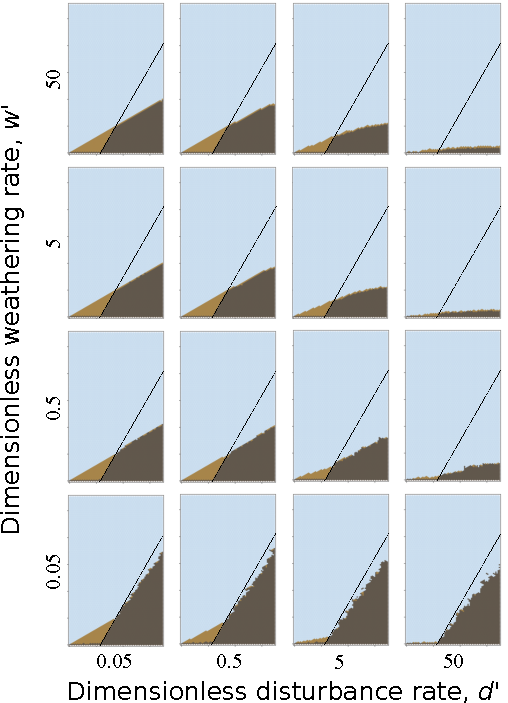
\includegraphics[scale=1.5]{Figures/four_by_four_profiles_colluvial_wedge.pdf}}
\caption{Simulated facet profiles showing the development of a colluvial wedge (light brown cells) on the hangingwall.}
\label{fig:colluv}
\end{figure}


\subsection{Baselevel Change}

Up to now we have assumed that the baselevel elevation remains fixed to the rocks in the hangingwall. In real extensional systems, however, this will rarely be the case. With the hangingwall rock as a reference frame, baselevel may rise as the hangingwall basin undergoes aggradation: a common situation in extensional systems. On the other hand, if the entire extensional system rises relative to an external baselevel such as eustatic sea level, the hangingwall blocks may themselves be incised, such that the local baselevel within a given hangingwall falls. Hangingwall incision has occurred, for example, in parts of the central Apennines extensional province in Italy \citep[e.g.,][]{dagostino2003interactions}.

To explore how baselevel rise might influence facet evolution, we performed a series of models runs identical to those in the previous section, but with the addition of a numerical ``sill'' along the left boundary (Figure~\ref{fig:baselevelrise}). The sill's elevation rises through time at 25\% of the vertical speed of footwall motion. The experiment is imperfect, as there is no easy way to keep the facet length constant. Nonetheless, the results illustrate potential impacts of hangingwall aggradation. In the reference frame of hangingwall bedrock, the fault trace rises and migrates away from the basin. Aggradation reduces the gradient of both the bedrock facet and the colluvial wedge. When $w'$ and facet length are sufficiently low, the rate of accommodation space creation outpaces the sediment flux from the eroding facet, and all the incoming sediment is trapped (Figure~\ref{fig:baselevelrise}). In these cases, sediment from an external source, such as an axial river or a nearby fan fed by a transverse stream, might be expected to fill the extra accommodation space, creating a sharp contact between the facet and the (relatively flat) basin floor, with the fault trace essentially at the slope base, as is sometimes observed (for example, Figure~\ref{fig:facets}f). 

% DEJH This is great!

\begin{figure}[ht!]
\centerline{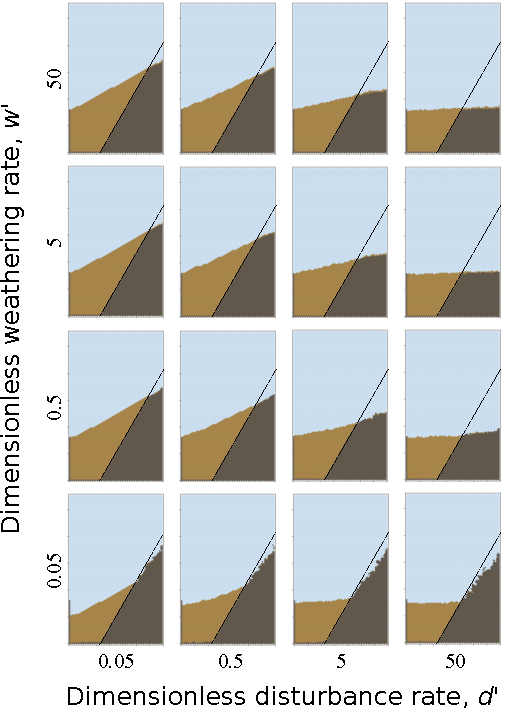
\includegraphics[scale=1.5]{Figures/four_by_four_profiles_baselevel_rise.pdf}}
\caption{Simulated facet profiles with a rising baselevel along the left model boundary, representing an aggrading hangingwall basin. The ``sill'' that implements rising baselevel is shown by the dark points along the lower portion of the left side of each panel.}
\label{fig:baselevelrise}
\end{figure}

When the weathering and (especially) disturbance rates are high relative to slip rate, the model realizations produce nearly flat footwall and hangingwall topography (Figure~\ref{fig:baselevelrise}, top three rows of right-most column). Effectively, the footwall is planed off as it rises, with the debris accumulating in the adjacent basin.

\subsection{Relation between facet angle and erosion rate}

To examine the predicted relationship between erosion rate and facet dip angle, we define a dimensionless slope-averaged vertical erosion rate as $E_v' = E_v / \delta d$. The denominator represents the maximum rate of regolith removal by disturbance: it is the rate one would obtain if each disturbance triggers a ravel event that transports the disturbed material to the base of the slope. In other words, $E_v' = 1$ can be thought of as representing ``perfect'' nonlocal transport \citep[e.g.,][]{tucker2010trouble,dibiase2017slope,doane2018nonlocal}. Cases with $E_v'<1$ arise either when some displaced regolith remains on the slope (indicating local, diffusive-like transport), or when the regolith cover is incomplete. Cases with $E_v'>1$ indicate some degree of direct gravitational failure of regolith material. To understand how $E_v'>1$ is possible, recall that the model allows for spontaneous mobilization of stationary regolith wherever a regolith cell lies diagonally above an adjacent air cell \citep[][their Figures 14 and 15]{tucker2016celllab}. This rule represents the gravitational failure that results when grains are perched in a configuration that exceeds their friction angle (imagine, for example, placing a pebble on an angle-of-repose slope: the pebble rolls downhill simply because the gravitational force exceeds the frictional resistance, without the need for a disturbance event to mobilize it).

The predicted relationship between facet dip angle and $E_v'$ is shown in Figure~\ref{fig:eroslope}.  The figure depicts data from a set of model runs with varying weathering efficiency ($w$) and slip rate ($V$). Dotted lines connect runs with the same weathering efficiency but varying $V$; %, with $w$ ranging from $10^{-5}$ y$^{-1}$ to $10^{-2}$ y$^{-1}$. F
for each such set of points, slip rate rises progressively from left to right, accompanied by an increase in facet angle. Color shading in (a) indicates the proportional regolith cover at the end of each run, while shading in (b) shows the ratio of actual slope-normal erosion rate to the theoretical maximum that would apply if regolith were instantly removed as soon as it was created. 

The results illustrate two regimes of behavior. Regolith-mantled facets show a strongly nonlinear relationship between angle and erosion rate, with a rapid acceleration in erosion rate near the model's 30$^\circ$ angle of repose (yellow (light-colored) points in Figure~\ref{fig:eroslope}a). Rocky facets, on the other hand, have a roughly log-linear relationship (blue (dark) points in Figure~\ref{fig:eroslope}a).

\begin{figure}[ht!]
\centerline{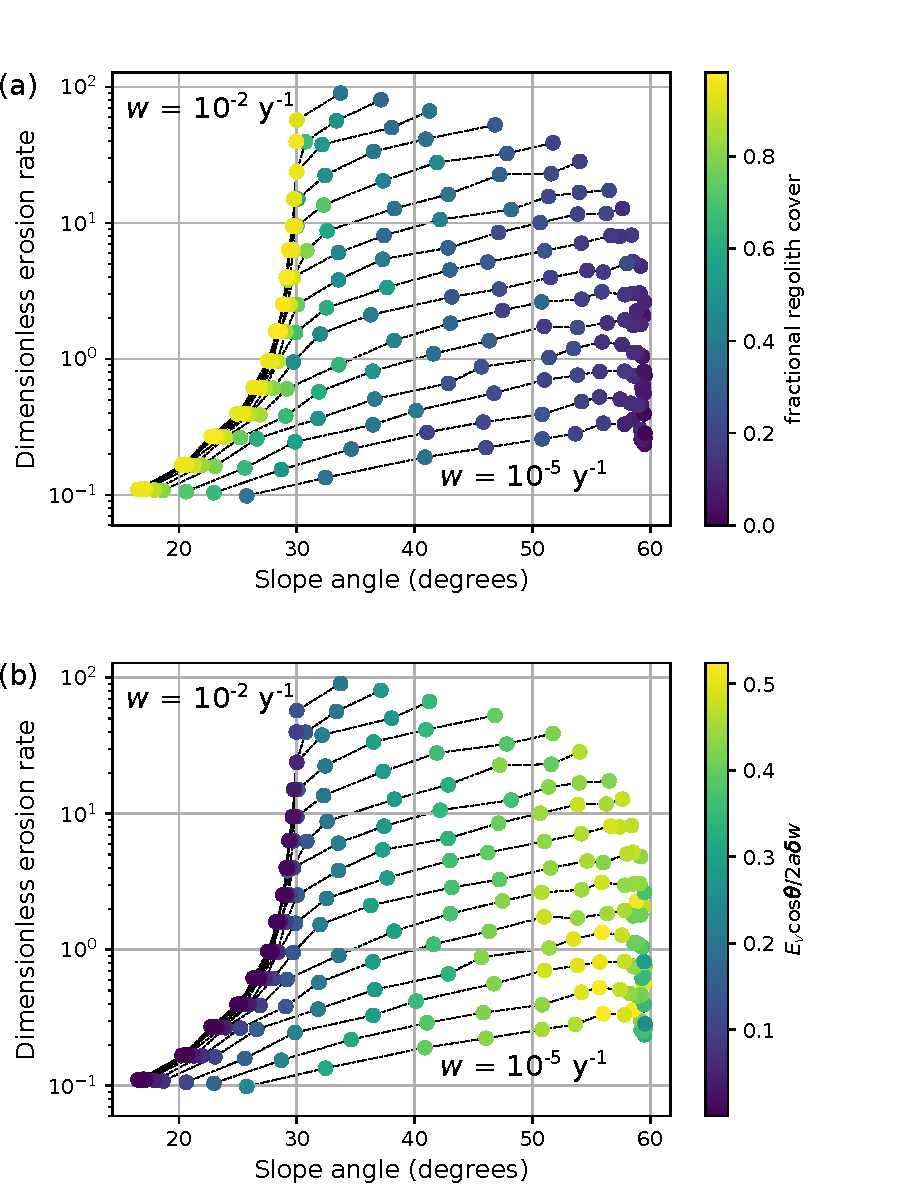
\includegraphics[scale=0.75]{Figures/ero_rate_vs_slope_angle.pdf}}
\caption{Relationship between dimensionless erosion rate and steady-state facet angle, generated from a set of model runs with varying $w$ (from $10^{-5}$ y$^{-1}$ to $10^{-2}$ y$^{-1}$), varying $\tau_s$ (from 10$^2$ to 10$^5$ y, corresponding to $V$ from 0.005 to 5 mm y$^{-1}$), and fixed $d$ ($10^{-4}$ y$^{-1}$). Each dashed line connects a series of runs with identical $w$ but varying $\tau_s$ (decreasing from left to right). Color in (b) represents the ratio of actual slope-normal erosion rate, estimated from the run's last snapshot, to the theoretical maximum. For very steep cases, the estimation of erosion rate relies on just a small number of eroded cells, and gives rise to variability in the erosion-rate ratio when angle is greater than about $50^\circ$. Color scales shown by bars to right of each figure.}
\label{fig:eroslope}
\end{figure}

The first regime represents transport-limited behavior. As slope angle increases, the model predicts a nonlinear increase in average erosion and transport rates, and a transition in morphology from convex-upward to planar \citep{tucker2018lattice}. For fully regolith-mantled slopes, the model's 30$^\circ$ effective angle of repose imposes an upper limit (yellow points in Figure~\ref{fig:eroslope}a). This behavior is consistent both with the Andrews-Bucknam transport law \citep{andrews1987fitting,roering1999evidence} and with experimental and field data on soil-mantled hillslopes \citep{roering2001hillslope,binnie2007tectonic,roering2008well,ouimet2009beyond,stock2009spatial,dibiase2012hillslope}.

The second regime represents weathering-limited behavior. In this regime, for a given weathering efficiency ($w$), the erosion rate rises approximately exponentially with slope angle, as indicated by the roughly linear trends for facets with less than $\sim$80\% regolith cover in Figure~\ref{fig:eroslope}a (note the logarithmic y-axis). The relationship reflects increased regolith mobility, and decreased cover fraction, on steeper slopes. Because of surface roughness, the regolith is not infinitely mobile, but rather can become temporarily trapped and stored in micro-depressions. These micro-depressions appear even on very steep simulated bedrock facets, like those along the bottom row of Figure~\ref{fig:dwprofiles}. One consequence is that the slope-normal erosion rate remains below  the theoretical maximum of $E_{max} = 2a\delta w$, which would represent a case of pure dissolution and no regolith production (symbol colors in Figure~\ref{fig:eroslope}b illustrate the ratio of actual erosion rate to this theoretical maximum). This weathering-limited regime illustrates an interesting feedback: weathering produces micro-topographic roughness features that trap colluvium, preventing slopes above the angle of repose from become completely bare and (according to the rules of the model) shielding some of the bedrock from weathering. As the slip rate increases, the ability of micro-topography to trap material is diminished, the fractional cover declines, and the erosion rate rises.


\section{Discussion}

\subsection{Understanding the variability of facet form}

Facets and their colluvial toes exhibit a fascinating variety of forms, with notable differences in slope angle, regolith cover, profile shape, and the presence or absence of a slope break at the fault trace. Although the process model developed here has only two dimensionless parameters ($w'$ and $d'$), it can reproduce much of the observed variety. The model manifests two general modes of behavior. Modeled slopes for which weathering efficiency is much greater than slip rate ($w' \gg 1$) exhibit transport-limited behavior, in which slope gradient is largely insensitive to weathering efficiency (Figure~\ref{fig:angw}, points with $w' > 1$). In this mode, the equilibrium dip angle for modeled facets with a slip rate greater than the characteristic rate of soil disturbance ($d' \le 1$) is the angle of repose ($30^\circ$ in the model) (Figure~\ref{fig:angw}, small circles and pluses at $w'>1$). When disturbance frequency exceeds the slip rate, facet slopes act as diffusion-like hillslopes, with concave-upward longitudinal profiles, and average dip angles below the angle of repose (illustrated by the upper right panels in Figure~\ref{fig:dwprofiles}, and by the stars and triangles at $w' > 1$ in Figure~\ref{fig:angw}). In either case, the facet's profile shape and dip angle are largely insensitive to weathering efficiency.

By contrast, facet slopes with a slip rate faster than the potential weathering efficiency ($w'<1$) operate in a weathering-limited mode. In this mode, dip angle depends on weathering efficiency, slip rate, and disturbance frequency (Figure~\ref{fig:angw}, points for $w'<1$). In this mode, facets are planar, and may be steeper or gentler than the angle of repose. Although weathering limits the rate of erosion in this mode, the processes of soil disturbance and downslope transport still exert an important influence; all else equal, facets with lower disturbance frequency are predicted to be steeper, and vice versa. The morphologic signature that most clearly distinguishes weathering-limited and transport-limited modes is the proportional regolith cover, which depends primarily on weathering efficiency and secondarily on disturbance frequency (Figure~\ref{fig:regw}).

The model also predicts that a break in slope between the facet surface and the colluvial apron below will occur either when the facet dip angle exceeds the angle of repose, or when the lack of regolith limits the transport and erosion rate on the facet (Figure~\ref{fig:colluv}).  Both cases occur in the weathering-limited regime, and are marked by an incomplete regolith cover on the facet. The slope break reflects a contrast in erosion and transport efficiency between the rocky facet surface and the colluvial wedge. For a system with a relatively steady baselevel, presence of a slope break suggests a weathering-limited regime. The converse is not quite true; model realizations in the transitional regime of $w'\approx d' \approx 1$ show only a subtle slope break that might be difficult to detect in the field, especially under baselevel rise (Figures~\ref{fig:dwprofiles} and \ref{fig:colluv}). 

A terrestrial laser scanning study of the Campo Felice fault in the Italian central Apennines provides an interesting case study of an active fault with a slope break between facet and colluvial wedge. A set of 25 topographic profiles collected by \citet{wilkinson2015slip} reveal a footwall slope angle of $40.3^\circ\pm 4.6^\circ$, with the colluvial wedge below dipping at $35.7^\circ\pm3.2^\circ$. The facet surface on the footwall is rocky, with a colluvial cover fraction that we estimate from a reconnaissance survey to be $\approx 80$\%. Both the slope break and the incomplete colluvial cover imply a weathering-limited regime. 

Similarly, field observations of facets along the Wasatch fault zone are also consistent with the model. Where slopes are below the angle of repose, bedrock breaks the surface only rarely, and no slope break is seen between facet and wedge. Where facet angles reach and begin to exceed likely angles of repose, bedrock exposure becomes much more obvious, but also highly spatially variable. This is accompanied by the appearance of a distinct break in slope between the facet and the wedge. These observations suggest a transition from the $w' > 1$ to $w' < 1$ domains, presumably driven by spatial variation in fault slip rate on different segments of the fault.

\subsection{Tectonics from process and topography}

The two-parameter cellular model implies a systematic relationship between facet angle, regolith cover, and erosion rate. For fully regolith-covered slopes, the model's behavior is broadly consistent with the Andrews-Bucknam transport law, which expresses a nonlinear relation between sediment flux per width, $q_s$, and slope gradient, $S$:
\begin{equation}
q_s = D_s S \left( \frac{1}{1-(S/S_c)^2} \right),
\label{eq:andrbuck}
\end{equation}
where $D_s$ [L$^2$/T] is a rate coefficient and $S_c$ is a threshold slope. The key difference is that whereas equation~(\ref{eq:andrbuck}) diverges at $S=S_c$ (and therefore only applies when $S<S_c$), the cellular model implies the possibility that $S$ can exceed $S_c$. The transition from below-threshold to above-threshold form coincides with a shift from soil-mantled to partly rocky, and represents a limitation on regolith transport as the cover thins. The limitation has two elements. First, the reduction in cover limits the degree of mobilization by disturbance. Second, microtopography limits the transport length of disturbed particles, and effectively traps regolith even when the overall slope angle exceeds the angle of repose. Both effects must occur on real hillslopes. Capturing them with a geomorphic transport law may require a nonlocal formulation that replaces the divergence in the Andrews-Bucknam law with a reduction in transport rate as regolith cover shrinks. One potential approach would be an explicit representation of characteristic transport length, which would vary both with $S/S_c$ and with the ratio of mean regolith thickness to bedrock roughness.

Another way to envision the slope-erosion relation is to consider a set of facets with identical lithology and climate (and hence fixed $W$ and $D$) but varying slip rate (Figure~\ref{fig:slopeslip}). Facets with a lower rate of slip would tend to be fully regolith mantled (unless $W$ is especially low), and for this subset, increasing slip rate would be met with a strongly nonlinear increase in facet angle (Figure~\ref{fig:slopeslip}, yellow (light-colored) points). Once the angle comes close to the threshold angle for colluvium, any further increases in slip rate would be accompanied by an increase in gradient above the threshold angle, and a reduction in colluvial cover fraction (Figure~\ref{fig:slopeslip}, dark-colored points).

\begin{figure}[ht!]
\centerline{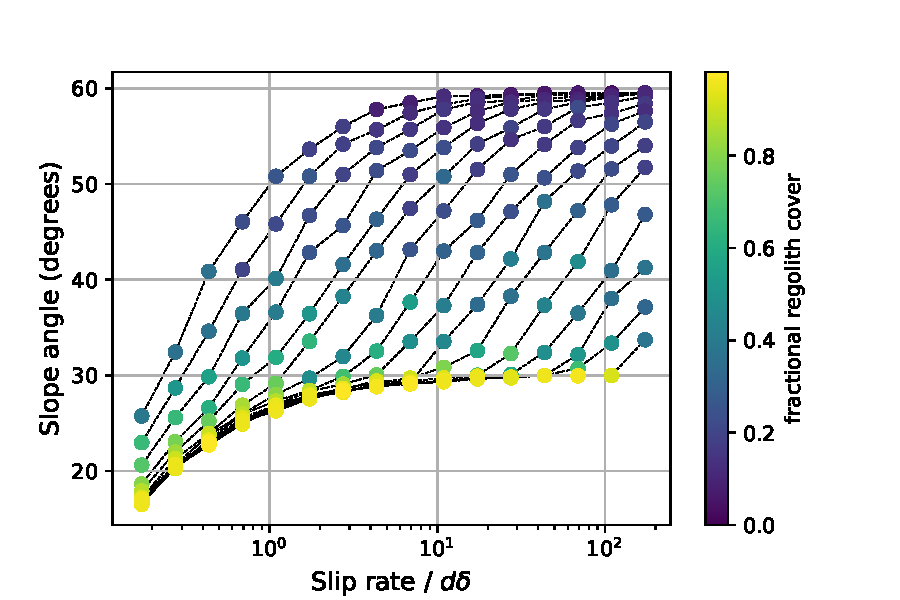
\includegraphics{Figures/slope_angle_vs_slip_rate_by_frac_soil.pdf}}
\caption{Relationship between steady-state facet angle and dimensionless slip rate, generated from the set of model runs shown in Figure~\ref{fig:eroslope}. Each dashed line connects a series of runs with identical $W$ but varying $V$.}
\label{fig:slopeslip}
\end{figure}

The cellular model suggests an interesting role for topographic roughness. The stochastic nature of weathering and regolith-disturbance events creates surface roughness, and especially so when a substantial fraction of rock is exposed at the surface (Figures~\ref{fig:dissruns} and \ref{fig:dwprofiles}). The development of roughness can accelerate rock weathering because it increases the exposed surface area. At the same time, as noted above, a rough surface can trap and hold regolith even when the average slope angle is well above the angle of repose, which allows even very steep slopes to retain some degree of regolith cover. On vegetated hillslopes, vegetation also contributes to sediment trapping \citep{dibiase2013vegetation,doane2018nonlocal}. In the model, trapping of regolith by roughness elements retards weathering by shielding the rock. In reality, it is possible that a thin regolith cover could actually accentuate rock weathering by trapping chemically reactive water and/or enhancing plant growth and vegetation-related weathering, as hypothesized by \citet{gilbert1877report}. The consequences of such an effect for facet evolution might be explored numerically with a modified version of the cellular model that allows faster weathering for rock in contact with near-surface regolith.

%\deleted{To the extent that the cellular model provides a reasonable analogy for real facets, its behavior suggests an explanation for why many facets show dip angles in the range of 32--40$^\circ$: that facets often weather sufficiently rapidly to approach a threshold angle for stability, consistent with the hypothesis of \citet{blackwelder1928recognition}. The models explored here also implies that the occurrence of facets considerably steeper than 40$^\circ$ requires a weathering efficiency (maximum weathering rate) less than the rate of fault slip (in other words, $w'<1$).}\explain{I've shifted this down to where I think it fits better}

One indicator of relatively efficient weathering is the presence of a more or less complete soil mantle. Such soil-mantled facets clearly exist, as documented for example by \citet{menges1990soils}. Given that slip rates on faceted mountain fronts are commonly 0.1--2 mm/y \citep{depolo2000estimating}, an implication is that maximum rates of rock weathering on facets can be at least this high. Rates on that order are broadly consistent with the findings of \citet{heimsath2012soil}, who demonstrated  that regolith production tends to be faster on steeper slopes.

%\deleted{The range in dip angles among facets may provide indirect information about rates of rock weathering. Active normal faults are often adorned with well-preserved bedrock scarps several meters high, with dip angles equivalent to the fault dip. Yet complete facet slopes are rarely steeper than about 40$^\circ$, again suggesting that weathering rates averaged over the O(10$^5$) years required to create a mountain front are comparable to or greater than the slip rate.}\explain{Not sure this was adding much that wasn't said earlier. Maybe talk about the scarps explicitly, but not in this context?}

To test the idea that facet angle and soil cover depend on rates of weathering and fault slip, one place to look would be extensional systems in a hyper-arid environment. In such an environment, faults slipping at millimeters per year would be expected to produce rocky facets steeper than the threshold angle for granular material, all else equal. The same could be said of facets formed in highly resistant lithologies such as quartzite.

One limitation to scenarios that considered here regards the potential role of partial dissolution in soluble lithologies. For example, carbonates underlie many of the prominent facets in the Mediterranean region, and facets we have surveyed in central Italy often host a thin (order 10~cm) and discontinuous soil cover \citep{tucker2011geomorphic}. Copious clastic debris in fans and colluvial wedges implies that mechanical weathering plays a major role, but it is also possible that partial dissolution of hillslope colluvium results in a soil cover that is thinner than it otherwise would be (it is also conceivable that the soils have thinned over historic time as a result of heavy grazing).

The behavior of the cellular model is consistent with a geometric model that relates facet angle to fault dip and the ratio of slope-normal erosion rate to slip rate (equation~\ref{eq:predangle}). An important caveat in applying this model is that the erosion rate can be expected to vary systematically with slope angle, even on weathering-limited slopes. The cellular model predicts that the relationship between erosion rate and slope angle depends on the degree of regolith cover, with transport-limited slopes showing a nonlinear relationship in which erosion rate rises rapidly as the threshold angle is approached, and weathering-limited slopes exhibiting a gentler, exponential-like relationship (Figure~\ref{fig:eroslope}). Hillslopes can transition from transport-limited to weathering-limited under changes in slip rate, as might be seen along strike in major normal fault systems, or with variation in weathering and transport efficiency through time under a changing climate. For all but the most strongly weathering-limited systems, this transition creates a notable kink in erosion rates close to the angle of repose, but whose exact form will be challenging to constrain from field observations alone. This kink also in part explains the tendency of real facets to show dip angles clustered in the range of 32--40$^\circ$: in this range, changes of only a few degrees can accommodate large changes in erosion rate, creating a geometric attractor state in this window. The occurrence of facets considerably steeper than 40$^\circ$ requires a weathering efficiency (maximum weathering rate) less than the rate of fault slip (in other words, $w'<1$). However, where this does occur, it is likely that facets offer records of past slip rates.

\subsection{Testable predictions}

The prediction that erosion rates exhibit significant and highly nonlinear variations with facet slope could be tested by obtaining erosion-rate estimates from facets above faults with an independently known slip rate, perhaps using cosmogenic radionuclide methods. The model suggests that the form of this relationship will be challenging to predict \textit{a priori} for a given environment from field observations of slope and bedrock exposure alone (e.g., Figure~\ref{fig:eroslope}). However, given independent constraints on actual erosion rates across the full range of slopes in a given facet array, the model suggests the potential to quantify fault slip rate from facet form. Methods that assume either a constant erosion rate or an Andrews-Bucknam style slope threshold will both result in poor calibration of slip rate from facet slope. %\deleted{One would need to sample facets with varying dip angle but uniform lithology. Ideally, the samples would include both soil-mantled and rocky sites. A method that could shed light on seasonal to annual transport rates on these steep surfaces would be monitoring of sediment traps, in which sediment accumulation over time could be remotely estimated with time-lapse cameras.}\explain{This comes across didactically, and might irritate people. They can figure this out themselves. It also invites the reviewer comment "So why didn't you do it?"}}

The predicted correlation between facet angle and fractional rock exposure should also be testable. In fact, recent work using lidar topography data has identified correlations between bedrock exposure and variables such as drainage density, erosion rate, fracture density, and mean slope gradient  \citep{dibiase2012hillslope,dibiase2018fracture,rossi2020orographic}. One challenge is that bedrock exposure metrics tend to rely on local slope gradient as a proxy, which carries the risk of spurious correlation. Overcoming this risk would require a slope-independent bedrock exposure proxy, such as one based on photographic imagery rather than topography.



\subsection{Model applications and limitations}

The cellular model we have explored has the advantage of simplicity (just two dimensionless parameters, $w'$ and $d'$), as well as a treatment of soil transport that honors its episodic and stochastic nature. Nonetheless, there are plenty of limitations. In terms of geomorphic process, the model assumes that transport and erosion by overland flow are negligible. This assumption may be justified for the planar, unincised cases that we address here, but is clearly not applicable to facets that are sliced by gully networks. We have also not considered the potential role of deep-seated landsliding in limiting the relief of facets on fast-slipping faults, though as noted earlier, this process does not seem to be especially common. In terms of tectonic processes, we have ignored both fault-plane rotation, and the possibility that the near-surface fault plane dip might not be identical to the long-term slip direction (for example, in softer material, the near-surface fault dip may effectively be steeper than the slip orientation; e.g., \citet{mccalpin2009paleoseismology}). We have also ignored the possibility of time-varying fault motion, which as \citet{hamblin1976patterns} suggested, might leave an imprint on mountain-front morphology. In terms of geomorphic processes, the analysis has been restricted to slopes governed by creep and ravel, as opposed to wash or landsliding. Similarly, we have not addressed transient facet growth, fault breccia (or other forms of lithologic heterogeneity), varying fault dip, the occurrence of multiple parallel faults, or the effect of a basinward shift in the position of the active range-bounding fault. These and other effects could be explored theoretically using the cellular framework, which could in turn point toward additional field-testable predictions.

Questions concerning the formation and evolution of bedrock fault scarps could be addressed by incorporating discrete slip events, as opposed to the quasi-continuous slip considered here. Used in that fashion, the model could provide a useful tool for analyzing and interpreting cosmogenic radionuclide samples on bedrock fault scarps. The numerical model could also provide a template for developing an improved continuum theory of soil transport on steep slopes: one that overcomes the limited range of applicability of the Andrews-Bucknam law, and accounts for the role of microtopography in trapping sediment, and the role of bedrock exposure in limiting downslope sediment flux.


%[TO DO: THINK ABOUT WHAT THE LAW MIGHT LOOK LIKE, AND THE COEFFICIENTS]

%1 - can a model that combines rock weathering with disturbance-driven soil creep account for the observed range in facet angle, regolith cover fraction, shape, and colluvial wedge angle? If so, what are the primary controlling factors?  yes: runs show variation in angle, reg cover, shape, and colluv angle. all are controlled by two dimensionless params.

%2 - Does the model imply a systematic relationship between facet angle and erosion rate, and if so what does that relationship look like? yes, sort of. the implication is that behavior differs between mantled and rocky facets. mantled ones show a nonlinear curve consistent with andrews-bucknam, but instead of blowing up at S=Sc it transitions to partial cover.

%3 - surface roughness plays a role. can accelerate rock weathering by exposing more surface area, but also retard (?) weathering by shielding rock. (could explore dynamics by making an near-surface regolith type, and having a rule for fast weathering when that touches rock)

%4 - how does the model compare to what we see in nature? one thing it suggests is that facets near angle of repose should be common, and indeed they seem to be. on the other hand, facets with angle above 40 deg seem to be quite rare, limited to cliffs interspersed with gentler segments. maybe that's where deep-seated landsliding comes in. mantled facets certainly exist, as in menges case study and our own obs from wfs. rocky ones too, as in italy (assuming it isn't goats). the rarity of very steep facets (with the possible exception of facets formed in basalt). seems to imply that potential rates of bedrock weathering outpace slip rates nearly everywhere. because sustained slip rates of 1 mm/yr or more are common, this in turn suggests potential rates of weathering even higher than that. seems to contradict heimsath and friends data, and we don't know why. a place to test would be hyper-arid and/or hyper-cold extensional systems.

% DEJH: Interestingly, I have been looking at some NUTS facets in Uganda. The walls of the East African Rift there can reach 50deg. Unfortunately, couldn't approach to see condition of the hillslopes, just view across the valley in haze - but presumably they are rocky. This in an environment with *extreme* weathering rates as well. I remain a little perplexed about this. It's possible there's a role for the (deep?) Lake Albert which abuts the facet for most of its length. Does this create odd base level effects?

%5 - one implication is that the geometric model, one can't transfer it among sites with different theta without accounting for a change in erosion rate. if you assumed a fixed erosion rate among a population of facets, it would underestimate the differences in slip rate represented by variations in angle.

%DEJH: #5 is important but not well emphasised. This is why I suggested an explicit U vs S figure further up. I've also modified a chunk of the discussion to emphasise this explicitly.

%6 - we haven't accounted for lots of things. fault rotation near surface. wash. deep-seated landsliding. possibility that weathering accelerates under a thin cover, rather than being reduced. basalt landscapes.

%7 - test model prediction with cosmo nuclides: how much does erosion rate actually vary with gradient within a given lithology, or with lithology for a given gradient? one could get a sense of short-term erosion and transport rates with methods as simple as sediment fences. this could help establish transport mechanisms (ravel vs wash for example).

%8 - we've deliberately kept it simple, but model could be used to explore predictions about stuff like episodes of slip and quiescence, multiple fault strands, variation in lithology

%A THING TO PLAY WITH: IS THERE A MATHEMATICAL FORM THAT ASYMPTOTES SORT OF TO ANGLE OF REP BUT THROTTLES TO FINITE UNDER LIMITED SOIL COVER? TRY PLOTTING ERO RATE VS SOIL COVER

\section*{Conclusions}

The longitudinal profiles of normal-fault facets show a wide diversity in form. Facets can vary in slope angle from several degrees to over $40^\circ$. Soil entirely blankets some of them, while others reveal bare rock with a patchy colluvial cover. Some show a distinct slope break between the facet and the colluvial wedge below, while others exhibit a continuous, uniform gradient across the fault trace from footwall to basal colluvium. Many have gradients close to a threshold angle for colluvium, but many others dip more gently.

A stochastic cellular automaton model of hillslope evolution with two dimensionless parameters can account for the observed diversity in longitudinal profile form. The model addresses the morphotectonic evolution of the near-surface portion of the footwall of a $60^\circ$-dipping active normal fault. It uses transition rules to represent bedrock weathering,  and the intermittent disturbance and transport of regolith. As shown in previous work, the model's parameters have a physical meaning and can be related to the more common parameters of geomorphic transport laws for regolith production and downslope transport. The two dimensionless process parameters represent characteristic velocities for weathering and regolith disturbance, respectively, normalized by the fault slip rate.

The model exhibits two modes of behavior: transport-limited and weathering-limited. Under the former regime, which represents relatively large weathering efficiency, facet angle depends on disturbance frequency and fault slip rate. Regolith fully blankets the modeled facets, and the threshold angle for granular-material failure imposes an upper limit to gradient. This soil-mantled, threshold behavior emerges when the potential weathering rate exceeds the fault slip rate, but the slip rate outpaces the disturbance rate. In this regime, modeled slopes show a continuous gradient across the fault trace, from colluvial wedge to footwall.

Weathering-limited behavior occurs when the fault-slip rate exceeds the maximum regolith production rate. Modeled facets in this regime show intermittent regolith cover, with the cover percent depending mainly on the ratio of (potential) weathering and slip rates, and secondarily on disturbance frequency. Gradient may exceed the threshold angle for colluvium; in this case, a partial colluvial cover remains held in place by microtopography. If weathered rock dissolves instead of transitioning to mobile regolith, the model recaptures a geometric analytical solution for facet angle as a function of the ratio of erosion to slip rate. Under weathering-limited behavior, modeled facets can exhibit a slope break between footwall and colluvial wedge when either the footwall slope exceeds the threshold angle, or disturbance frequency is sufficiently high (or slip rate sufficiently low) to transport eroded material at a lower-than-threshold gradient. Despite the term, the model's weathering-limited mode involves important interactions between weathering and regolith transport processes. For example, the rate of erosion in this mode depends on regolith disturbance frequency, which helps set the degree of rock exposure.

The model predicts a nonlinear relation between erosion rate and gradient. The nature of the relation depends on the mode. A soil-mantled, transport-limited facet slope shows a nonlinear curve that resembles the Andrews-Bucknam transport law, with a nonlinear approach to an asymptote at the threshold angle for stability. But where the Andrews-Bucknam law diverges at the threshold angle and says nothing about what happens above it, the cellular model implies a transition to weathering-limited behavior when gradient exceeds the threshold. For rocky, weathering-limited slopes, the model predicts an exponential-like relation between erosion rate and gradient.

The degree to which the model provides an accurate representation of facet profile evolution remains to be tested. Estimating the erosion rates on facets of varying angle, lithology, and soil cover using cosmogenic nuclide analysis could provide a test of the predicted controls on erosion rate. Direct collection and measurement of downslope sediment flux could provide a shorter-term test that might also illuminate the governing regolith production and transport processes. Ultimately, such data, in combination with the process-based model presented here (or a suitably modified version thereof) could provide the basis for a geomorphic transport law that captures the transition in behavior across the threshold angle for soil stability, and the related transition from soil-mantled to rocky slopes.

% DEJH final thoughts. 1. I think a plot of U vs E for multiple, constant w, d (i.e., sensibly evolving w’, d’) would prove valuable insight for the tectonically-minded reader. 2. What happens if w & d aren't independent of S? 3. The form of the trend in Fig 12 deserves a bit more attention, as you note above. I think simply describing it as log-linear or exponential might be unwise, since the sigmoid transition from Andrews-B style to actually exponential happens right where it matters. This is of course what creates the clustering of facets close to and just above the angle of repose - we said that already, but I've tried to tweak things to make it more obvious. This links to (1), in that the implication is that *for the same mountain front, with the same w and d,* erosion rates vary between facets, and we get evolution between the styles of facet your talking about in the text (c.f., wasatch). 4. Figs 7, 10, 11 all deserve full pages; they're too small as they are.








%Outline 
%
%
%I. Introduction
%
%Morphology of normal-fault facets poses some interesting questions:
%- variations in facet dip angle (from less than 10 degrees to over 30 degrees)
%- despite planar morphology, dip angle of facet is almost always less than the dip angle of the fault
%- some facets are mantled by a mostly continuous mantle of soil, whereas others are rocky and host discontinuous, patchy soil
%- in some cases, the mapped fault trace lies at the base of the facet, where in others, the fault trace occurs in mid-slope, coinciding with a transition from rock to colluvium but without a clear break in slope
%
%Literature review: facets have intrigued geoscientists both because of their striking morphology, and because of what they can reveal about tectonic motion and earthquake hazards. Various refs: Carole Petit, McCalpin, Tucker et al., 2011, etc., etc.
%
%Need a process-based model that can account for the basic morphology of facets, and the key variations in morphology that are observed.
%
%
%II. Normal-Fault Facets in the Italian Central Apennines and the central western United States
%
%Show photos, lidar images, for facets in Wasatch and north, and in Italy
%
%
%III. Cellular Model of Facet Evolution
%
%A. Why a Cellular Model?
%
%motivation for using this kind of model, citing Grain Hill paper and noting that process params can be pinned
%
%B. Model Description
%describe model

%C. Experimental Design
%
%goal is to determine:
%- what are the necessary and sufficient conditions to reproduce the common morphology of a facet: planar with thin soil cover?
%- can the model account for observed range in facet morphology and soil cover?
%- what are the key controls on slope gradient, profile shape, and regolith cover fraction and thickness?


%IV. Results
%
%A. Weathering-limited facets
%
%demonstrate that one recaptures Tucker et al. 2011 behavior when d' >> w': experiments in which the predicted angle should be 60 degrees (no weathering), 45, 30, 15.
%
%B. Influence of d' and w'
%
%3x3 (or maybe 5x5) plot in d' and w' space
%
%plot of facet dip angle in d' and w' space (from talk, showing family of curves)
%
%C. (optional) what if rock or soil can dissolve, a la Italian carbonates? (dissolution rule)
%
%D. (optional) baselevel effects - what happens when either you have a basal stream cutting down or a hangingwall valley aggrading? This would require having a modification that would add or remove rock cells along the left edge

%E. what sets the effective E vs S relation? refer back to T et al., 2011, noting restrictive assumption of slope-independent erosion rate

%F. (optional) how could one mimic the effective rule in a differential equation world? Try out something like the depth-dependent Taylor model.


%V. Discussion

%- model accounts for basic morphology and shape. necessary and sufficient conditions for planar facet with dip angle less than fault dip: weathering of rock plus disturbance, and [something about limits, i.e., curvature appears when $d'/w' >$ ...]

%- facet angle close to angle of repose is an attractor state, because below that angle, the transport rate and length scale of produced regolith goes way down

%- for this reason, it should be common to observe cases where the fault trace cuts across a roughly uniform slope, marking a transition from eroding rock to aggrading colluvium

%- cases that do NOT show this morphology are anomalies, likely reflecting strong baselevel control apart from simply fault slip (aggradation or incision)

%- facet dip angle is set by ...

%- facet soil cover depth and spatial continuity set by ...

%- facets are predicted to become concave-up when ...

%- to test these ideas, we need cosmos on facet slopes!


%VI. Conclusions

%model accounts for facet morphology as a consequence of tectonic motion, rock weathering and regolith disturbance

%variations in facet morphology can be explained as a consequence of ...

%erosion rate does depend on slope gradient, like thus-and-such

%need cosmos to test these predictions






%% Enter Figures and Tables near as possible to where they are first mentioned:
%
% DO NOT USE \psfrag or \subfigure commands.
%
% Figure captions go below the figure.
% Table titles go above tables;  other caption information
%  should be placed in last line of the table, using
% \multicolumn2l{$^a$ This is a table note.}
%
%----------------
% EXAMPLE FIGURE
%
% \begin{figure}
% \end{figure}










%% ------------------------------------------------------------------------ %%





%%% End of body of article

%%%%%%%%%%%%%%%%%%%%%%%%%%%%%%%%
%% Optional Appendix goes here
%
% \appendix resets counters and redefines section heads
% but doesn't print anything.
% After typing \appendix
%
%\section{Here Is Appendix Title}
% will show
% A: Here Is Appendix Title
%

%%%%%%%%%%%%%%%%%%%%%%%%%%%%%%%%%%%%%%%%%%%%%%%%%%%%%%%%%%%%%%%%
%
% Optional Glossary, Notation or Acronym section goes here:
%
%%%%%%%%%%%%%%
% Glossary is only allowed in Reviews of Geophysics


%
%%%%%%%%%%%%%%
% Acronyms
 

%
%%%%%%%%%%%%%%
% Notation




%%%%%%%%%%%%%%%%%%%%%%%%%%%%%%%%%%%%%%%%%%%%%%%%%%%%%%%%%%%%%%%%
%
%  ACKNOWLEDGMENTS

\acknowledgments
This research was supported by the U.S.\ National Science Foundation (NSF) Earth Sciences Division (EAR-1349390). The numerical modeling was facilitated by the Community Surface Dynamics Modeling System (CSDMS; NSF EAR-1831623), and by the NSF Office of Advanced Cyberinfrastructure (OAC-1450412).


%%  REFERENCE LIST AND TEXT CITATIONS
%
% Either type in your references using
%
% \begin{thebibliography}{}
% \bibitem{}
% Text
% \end{thebibliography}
%
% Or, to use BibTeX:
%
% Follow these steps
%
% 1. Type in \bibliography{<name of your .bib file>}
%    Run LaTeX on your LaTeX file.
%
% 2. Run BiBTeX on your LaTeX file.
%
% 3. Open the new .bbl file containing the reference list and
%   copy all the contents into your LaTeX file here.
%
% 4. Run LaTeX on your new file which will produce the citations.
%
% AGU does not want a .bib or a .bbl file. Please copy in the contents of your .bbl file here.



%\bibliography{gt_library.bib}

\begin{thebibliography}{41}
\providecommand{\natexlab}[1]{#1}
\expandafter\ifx\csname urlstyle\endcsname\relax
  \providecommand{\doi}[1]{doi:\discretionary{}{}{}#1}\else
  \providecommand{\doi}{doi:\discretionary{}{}{}\begingroup
  \urlstyle{rm}\Url}\fi

\bibitem[{\textit{Anderson}(1977)}]{anderson1977compound}
Anderson, T.~C. (1977), {Compound faceted spurs and recurrent movement in the
  Wasatch Fault zone, north central Utah}, Ph.D. thesis, Brigham Young
  University.

\bibitem[{\textit{Andrews and Bucknam}(1987)}]{andrews1987fitting}
Andrews, D., and R.~C. Bucknam (1987), Fitting degradation of shoreline scarps
  by a nonlinear diffusion model, \textit{Journal of Geophysical Research},
  \textit{92}(B12), 12,857--12,867.

\bibitem[{\textit{Binnie et~al.}(2007)\textit{Binnie, Phillips, Summerfield,
  and Fifield}}]{binnie2007tectonic}
Binnie, S.~A., W.~M. Phillips, M.~A. Summerfield, and L.~K. Fifield (2007),
  Tectonic uplift, threshold hillslopes, and denudation rates in a developing
  mountain range, \textit{Geology}, \textit{35}(8), 743--746,
  \doi{10.1130/G23641A.1}.

\bibitem[{\textit{Blackwelder}(1928)}]{blackwelder1928recognition}
Blackwelder, E. (1928), The recognition of fault scarps, \textit{The Journal of
  Geology}, \textit{36}(4), 289--311.

\bibitem[{\textit{Boulton and Whittaker}(2009)}]{boulton2009quantifying}
Boulton, S., and A.~Whittaker (2009), Quantifying the slip rates, spatial
  distribution and evolution of active normal faults from geomorphic analysis:
  Field examples from an oblique-extensional graben, southern turkey,
  \textit{Geomorphology}, \textit{104}(3-4), 299--316,
  \doi{10.1016/j.geomorph.2008.09.007}.

\bibitem[{\textit{Cotton}(1950)}]{cotton1950tectonic}
Cotton, C.A. (1950), Tectonic scarps and fault valleys,
  \textit{Geological Society of America Bulletin}, \textit{61}, 717--758.

\bibitem[{\textit{Bubeck et~al.}(2015)\textit{Bubeck, Wilkinson, Roberts,
  Cowie, McCaffrey, Phillips, and Sammonds}}]{bubeck2015tectonic}
Bubeck, A., M.~Wilkinson, G.~P. Roberts, P.~Cowie, K.~McCaffrey, R.~Phillips,
  and P.~Sammonds (2015), {The tectonic geomorphology of bedrock scarps on
  active normal faults in the Italian Apennines mapped using combined ground
  penetrating radar and terrestrial laser scanning}, \textit{Geomorphology},
  \textit{237}, 38--51, \doi{10.1016/j.geomorph.2014.03.011}.

\bibitem[{\textit{D'Agostino et~al.}(2003)\textit{D'Agostino, Jackson, Dramis,
  and Funiciello}}]{dagostino2003interactions}
D'Agostino, N., J.~Jackson, F.~Dramis, and R.~Funiciello (2003), {Interactions
  between mantle upwelling, drainage evolution and active normal faulting: an
  example from the central Apennines (Italy)}, \textit{Geophysical Journal
  International}, \textit{147}(2), 475--497,
  \doi{10.1046/j.1365-246X.2001.00539.x}.

\bibitem[{\textit{Davis}(1903)}]{davis1903mountain}
Davis, W.~M. (1903), The mountain ranges of the great basin, \textit{Harvard
  University Museum of Comparative Zoology Bulletin}, \textit{40}(3), 129--177.

\bibitem[{\textit{Davis}(1909)}]{davis1909geographical}
Davis, W.~M. (1909), \textit{Geographical Essays}, Ginn.

\bibitem[{\textit{Densmore et~al.}(1998)\textit{Densmore, Ellis, and
  Anderson}}]{densmore1998landsliding}
Densmore, A.~L., M.~A. Ellis, and R.~S. Anderson (1998), Landsliding and the
  evolution of normal-fault-bounded mountains, \textit{Journal of Geophysical
  Research}, \textit{103}, 15,203--15,219.

\bibitem[{\textit{DePolo and Anderson}(2000)}]{depolo2000estimating}
DePolo, C., and J.~Anderson (2000), Estimating the slip rates of normal faults
  in the great basin, usa, \textit{Basin Research}, \textit{12}(3-4), 227--240.

\bibitem[{\textit{DiBiase et~al.}(2012)\textit{DiBiase, Heimsath, and
  Whipple}}]{dibiase2012hillslope}
DiBiase, R., A.~Heimsath, and K.~Whipple (2012), Hillslope response to tectonic
  forcing in threshold landscapes, \textit{Earth Surface Processes and
  Landforms}, \doi{10.1002/esp.3205}.

\bibitem[{\textit{DiBiase and Lamb}(2013)}]{dibiase2013vegetation}
DiBiase, R.~A., and M.~P. Lamb (2013), Vegetation and wildfire controls on
  sediment yield in bedrock landscapes, \textit{Geophysical Research Letters},
  \textit{40}(6), 1093--1097, \doi{10.1002/grl.50277}.

\bibitem[{\textit{DiBiase et~al.}(2017)}]{dibiase2017slope}
DiBiase, R.~A., M.~P.~Lamb, V.~Ganti, and A.~M.~Booth (2013), Slope, grain size, and roughness controls on dry sediment transport and storage on steep hillslopes, \textit{Journal of Geophysical Research:
  Earth Surface},
  \textit{122}, 941--960, \doi{10.1002/2016JF003970}.

\bibitem[{\textit{DiBiase et~al.}(2018)\textit{DiBiase, Rossi, and Neely}}]{dibiase2018fracture}
DiBiase, R.~A., M.~W. Rossi, and A.~B. Neely (2018), {Fracture density and grain size controls on the relief structure of bedrock landscapes},
  \textit{Geology},
  \textit{46}(5),
  399--402.

\bibitem[{\textit{Doane et~al.}(2018)\textit{Doane, Furbish, Roering, Schumer,
  and Morgan}}]{doane2018nonlocal}
Doane, T.~H., D.~J. Furbish, J.~J. Roering, R.~Schumer, and D.~J. Morgan
  (2018), {Nonlocal sediment transport on steep lateral moraines, eastern
  Sierra Nevada, California, USA}, \textit{Journal of Geophysical Research:
  Earth Surface}, \textit{123}(1), 187--208, \doi{10.1002/2017JF004325}.

\bibitem[{\textit{Ellis et~al.}(1999)\textit{Ellis, Densmore, and
  Anderson}}]{ellis1999development}
Ellis, M., A.~Densmore, and R.~Anderson (1999), Development of mountainous
  topography in the basin ranges, usa, \textit{Basin Research}, \textit{11}(1),
  21--42.

\bibitem[{\textit{Fuller}(1931)}]{fuller1931geomorphology}
Fuller, R.~E. (1931), {The geomorphology and volcanic sequence of Steens
  Mountain in southeastern Oregon}, \textit{University of Washington
  Publications in Geology}, \textit{3}(1).

\bibitem[{\textit{Furbish et~al.}(2009)\textit{Furbish, Haff, Dietrich, and
  Heimsath}}]{furbish2009statistical}
Furbish, D., P.~Haff, W.~Dietrich, and A.~Heimsath (2009), Statistical
  description of slope-dependent soil transport and the diffusion-like
  coefficient, \textit{J. Geophys. Res}, \textit{114}, F00A05,
  \doi{10.1029/2009JF001267}.

\bibitem[{\textit{Gilbert}(1875)}]{gilbert1875report}
Gilbert, G. (1875), Report on the geology of portions of nevada, utah,
  california, and arizona: Us geog. and geol, \textit{Survey W. 100th Meridian
  Rept}, \textit{3}, 37--41.

\bibitem[{\textit{Gilbert}(1877)}]{gilbert1877report}
Gilbert, G. (1877), {Report on the geology of the Henry Mountains: US Geog. and
  Geol}, \textit{Survey, Rocky Mtn. Region}, \textit{160}.

\bibitem[{\textit{Gilbert}(1928)}]{gilbert1928studies}
Gilbert, G. (1928), \textit{Studies of basin-range structure}, \textit{U.~S.\
  Geological Survey Professional Paper}, vol. 153, United States Government
  Printing Office.

\bibitem[{\textit{Gilluly}(1928)}]{gilluly1928basin}
Gilluly, J. (1928), {Basin range faulting along the Oquirrh Range, Utah},
  \textit{Bulletin of the Geological Society of America}, \textit{39}(4),
  1103--1130.

\bibitem[{\textit{Hamblin}(1976)}]{hamblin1976patterns}
Hamblin, W. (1976), Patterns of displacement along the wasatch fault,
  \textit{Geology}, \textit{4}(10), 619.

\bibitem[{\textit{Heimsath et~al.}(2012)\textit{Heimsath, DiBiase, and
  Whipple}}]{heimsath2012soil}
Heimsath, A., R.~DiBiase, and K.~Whipple (2012), Soil production limits and the
  transition to bedrock-dominated landscapes, \textit{Nature Geoscience},
  \textit{5}(3), 210--214, \doi{10.1038/ngeo1380}.

\bibitem[{\textit{Knuth}(1955)}]{knuth1955potrzebie}
Knuth, D.E. (1955), Potrzebie system of weights and measures,
  \textit{Mad Magazine}, \textit{33}.

\bibitem[{\textit{Leeder and Jackson}(1993)}]{leeder1993interaction}
Leeder, M.R., and Jackson, J.A. (1993), {The interaction between normal faulting and drainage in active extensional basins, with examples from the western United States and central Greece}, \textit{Basin Research}, \textit{5}(2), 79--102.

\bibitem[{\textit{McCalpin}(2009)}]{mccalpin2009paleoseismology}
McCalpin, J. (2009), \textit{Paleoseismology}. Academic Press.

\bibitem[{\textit{Menges}(1990)}]{menges1990soils}
Menges, C. (1990), {Soils and geomorphic evolution of bedrock facets on a
  tectonically active mountain front, western Sangre de Cristo Mountains, New
  Mexico}, \textit{Geomorphology}, \textit{3}(3-4), 301--332.

\bibitem[{\textit{Ouimet et~al.}(2009)\textit{Ouimet, Whipple, and
  Granger}}]{ouimet2009beyond}
Ouimet, W.~B., K.~X. Whipple, and D.~E. Granger (2009), Beyond threshold
  hillslopes: Channel adjustment to base-level fall in tectonically active
  mountain ranges, \textit{Geology}, \textit{37}(7), 579--582,
  \doi{10.1130/G30013A.1}.

\bibitem[{\textit{Pack}(1926)}]{pack1926new}
Pack, F.~J. (1926), {New discoveries relating to the Wasatch fault},
  \textit{American Journal of Science}, \textit{11}(65), 399--410.

\bibitem[{\textit{Petit et~al.}({2009})\textit{Petit, Gunnell,
  Gonga-Saholiariliva, Meyer, and Seguinot}}]{petit2009faceted}
Petit, C., Y.~Gunnell, N.~Gonga-Saholiariliva, B.~Meyer, and J.~Seguinot
  ({2009}), {Faceted spurs at normal fault scarps: Insights from numerical
  modeling}, \textit{Journal of Geophysical Research---Solid Earth},
  \textit{{114}}, \doi{{10.1029/2008JB005955}}.

\bibitem[{\textit{Roering}(2008)}]{roering2008well}
Roering, J. (2008), {How well can hillslope evolution models ``explain''
  topography? Simulating soil transport and production with high-resolution
  topographic data}, \textit{Geological Society of America Bulletin},
  \textit{120}(9-10), 1248--1262, \doi{10.1130/B26283.1}.

\bibitem[{\textit{Roering et~al.}({1999})\textit{Roering, Kirchner, and
  Dietrich}}]{roering1999evidence}
Roering, J., J.~Kirchner, and W.~Dietrich ({1999}), {Evidence for nonlinear,
  diffusive sediment transport on hillslopes and implications for landscape
  morphology}, \textit{{Water Resources Research}}, \textit{{35}}({3}),
  {853--870}, \doi{10.1029/1998WR900090}.

\bibitem[{\textit{Roering et~al.}({2001})\textit{Roering, Kirchner, Sklar, and
  Dietrich}}]{roering2001hillslope}
Roering, J., J.~Kirchner, L.~Sklar, and W.~Dietrich ({2001}), {Hillslope
  evolution by nonlinear creep and landsliding: An experimental study},
  \textit{{Geology}}, \textit{{29}}({2}), {143--146},
  \doi{10.1130/0091-7613(2001)029<0143:HEBNCA>2.0.CO;2}.

\bibitem[{\textit{Rossi et~al.}(2020)\textit{Rossi, Anderson, Anderson, and
  Tucker}}]{rossi2020orographic}
Rossi, M.~.W., R.~S.~Anderson, S.~P.~Anderson, and G.~E.~Tucker (2020), Orographic controls on sub?daily rainfall statistics and flood frequency in the Colorado Front Range, USA, \textit{Geophysical Research Letters},
  \doi{10.1029/2019GL085086}.

\bibitem[{\textit{Schneider}(1925)}]{schneider1925discussion}
Schneider, H. (1925), {A discussion of certain geologic features of the Wasatch
  Mountains}, \textit{The Journal of Geology}, \textit{33}(1), 28--48.

\bibitem[{\textit{Stock et~al.}(2009)\textit{Stock, Frankel, Ehlers, Schaller,
  Briggs, and Finkel}}]{stock2009spatial}
Stock, G., K.~Frankel, T.~Ehlers, M.~Schaller, S.~Briggs, and R.~Finkel (2009),
  Spatial and temporal variations in denudation of the wasatch mountains, utah,
  usa, \textit{Lithosphere}, \textit{1}(1), 34--40, \doi{10.1130/L15.1}.

\bibitem[{\textit{Strak et~al.}(2011)\textit{Strak, Dominguez, Petit, Meyer,
  and Loget}}]{strak2011interaction}
Strak, V., S.~Dominguez, C.~Petit, B.~Meyer, and N.~Loget (2011), Interaction
  between normal fault slip and erosion on relief evolution: Insights from
  experimental modelling, \textit{Tectonophysics}, \textit{513}(1-4), 1--19,
  \doi{10.1016/j.tecto.2011.10.005}.

\bibitem[{\textit{Struble et~al.}(in review)\textit{Struble, McCoy, Hobley,
  Tucker, and Gregory}}]{struble2019mountain}
Struble, W.~T., S.~W. McCoy, D.~E.~J. Hobley, G.~E. Tucker, and L.~C. Gregory
  (in review), {Mountain-Front Facet Gradient Encodes Long-Term Slip Rate Along
  the Wasatch Normal Fault, USA}, \textit{TBD}.

\bibitem[{\textit{Tucker and Bradley}(2010)}]{tucker2010trouble}
Tucker, G., and D.~Bradley (2010), {Trouble with diffusion: Reassessing
  hillslope erosion laws with a particle-based model}, \textit{J. Geophys.
  Res}, \textit{115}.

\bibitem[{\textit{Tucker et~al.}(2011)\textit{Tucker, McCoy, Whittaker,
  Roberts, Lancaster, and Phillips}}]{tucker2011geomorphic}
Tucker, G., S.~McCoy, A.~Whittaker, G.~Roberts, S.~Lancaster, and R.~Phillips
  (2011), Geomorphic significance of postglacial bedrock scarps on normal-fault
  footwalls, \textit{Journal of Geophysical Research}, \textit{116}(F1),
  F01,022, \doi{10.1029/2010JF001861}.

\bibitem[{\textit{Tucker et~al.}(2016)\textit{Tucker, Hobley, Hutton,
  Gasparini, Istanbulluoglu, Adams, and Nudurupati}}]{tucker2016celllab}
Tucker, G.~E., D.~E. Hobley, E.~Hutton, N.~M. Gasparini, E.~Istanbulluoglu,
  J.~M. Adams, and S.~S. Nudurupati (2016), {CellLab-CTS 2015: continuous-time
  stochastic cellular automaton modeling using Landlab}, \textit{Geoscientific
  Model Development}, \textit{9}(2), 823--839, \doi{10.5194/gmd-9-823-2016}.

\bibitem[{\textit{Tucker et~al.}(2018)\textit{Tucker, McCoy, and
  Hobley}}]{tucker2018lattice}
Tucker, G.~E., S.~W. McCoy, and D.~E. Hobley (2018), A lattice grain model of
  hillslope evolution, \textit{Earth Surface Dynamics}, \textit{6}(3),
  563--582, \doi{10.5194/esurf-6-563-2018}.

\bibitem[{\textit{Wallace}(1978)}]{wallace1978geometry}
Wallace, R. (1978), {Geometry and rates of change of fault-generated range
  fronts, north-central Nevada}, \textit{Journal of Research of the U.S.\
  Geological Survey}, \textit{6}(5), 637--650.

\bibitem[{\textit{Wilkinson et~al.}(2015)\textit{Wilkinson, Roberts, McCaffrey,
  Cowie, Walker, Papanikolaou, Phillips, Michetti, Vittori, Gregory
  et~al.}}]{wilkinson2015slip}
Wilkinson, M., G.~P. Roberts, K.~McCaffrey, P.~A. Cowie, J.~P.~F. Walker,
  I.~Papanikolaou, R.~J. Phillips, A.~M. Michetti, E.~Vittori, L.~Gregory,
  et~al. (2015), {Slip distributions on active normal faults measured from
  LiDAR and field mapping of geomorphic offsets: an example from L'Aquila,
  Italy, and implications for modelling seismic moment release},
  \textit{Geomorphology}, \textit{237}, 130--141,
  \doi{10.1016/j.geomorph.2014.04.026}.

\bibitem[{\textit{Zuchiewicz and McCalpin}(2000)}]{zuchiewicz2000geometry}
Zuchiewicz, W.~A., and J.~P. McCalpin (2000), {Geometry of faceted spurs on an
  active normal fault: case study of the Central Wasatch Fault, Utah, USA}, in
  \textit{Annales Societatis Geologorum Poloniae}, vol.~70, pp. 231--249.

\end{thebibliography}





%%%%%%%%%%%%%%%%%%%%%%%%%%%%%%%%%%%%%%%%%
% Track Changes:
% To add words, \added{<word added>}
% To delete words, \deleted{<word deleted>}
% To replace words, \replace{<word to be replaced>}{<replacement word>}

% At the end of the document, use \listofchanges, which will list the
% changes and the page and line number where the change was made.

% When final version, \listofchanges will not produce anything,
% \added{} word will be printed, \deleted{} will take away the word,
% \replaced{}{} will print only the 2nd argument.

%%%
%\listofchanges
%%%


%the range-bounding faults themselves---observed in quarries or along bedrock tectonic scarps---

%, commonly in the range of , and the dip of the fault planes beneath, which 


%G.K.~Gilbert described triangular facets XXX. Their generally planar character, combined with their occurrence at or near the range-bounding fault, conveys the impression that they represent uplifted and exhumed fault planes. Commonly, however, facet slopes dip much more gently than the expected $\sim 60^\circ$ dip of a normal fault, implying erosional modification of the original fault plane.


%KEY IDEAS LINKED TO PAPERS:

%o Davis (1903, 1909) viewed facets as lightly modified exhumed fault planes, showing approximately the same dip as the fault itself. He reached this conclusion via the perception that facets along the WF have relatively little colluvium at their bases, even though there's no obvious means to remove colluvium. Gilbert (1928, but writing earlier) agreed: ``"the dip of the fault corresponds so nearly with the angle of rest that adjustment to stability involves little or no wasting."


%o The dip of facets is commonly in the range of 20--40o
%
%- Davis (1903, 1909): 32--40
%
%- Pack (1926) seldom more than 30
%
%- Blackwelder (1928) ``generally between 20 and 30 degrees, and rarely so much as 32''
%
%- Gilluly (1928) Lakes of Killarney fault 21--30o; Great Basin generally 25--35o; Genoa Peak, NV (quoting Lawson) 24o; Plum Ridge, OR (citing Gilbert) 34; Toyabe, NV, 20--35o
%
%- Fuller (1931) Steens is steep, but elsewhere in Great Basin usually about 30
%
%- Anderson (1977) 20--40, averaging around 35
%
%- Wallace (1978) 25--35, and also asserts that in fractured bedrock, angles in this range remain stable for 100kys, and views facets as relatively stable
%
%- Menges (1990) mean 20; can be lower
%
%- Petit (2009a) 22--38
%
%- Wilkinson (2015) 36 +/- 3


%o Dip of normal faults commonly 50--70o or more
%
%- Schneider (1925) Wasatch in quarry 72
%
%- Pack (1926) about 70 (Gilluly has him saying 60--75)
%
%- Blackwelder (1928) ``commonly between 50 and 90 degrees, and rarely less than 40 degrees''
%
%- Gilluly (1928) Lakes of Killarney fault: more than 60o; Genoa Peak, NV (quoting Lawson) 65; Plum Ridge, OR (citing Gilbert) 49; Toyabe, NV, 54, 59, 67
%
%- Fuller (1931) Oregon: 50--65, averaging about 60
%
%- Wallace (1978) 50--90
%
%- Wilkinson (2017) Campo Felice 57 +/- 4



%o Facets are much gentler than faults, so not simply exhumed fault planes
%
%- Pack (1926)
%
%- Blackwelder (1928)
%
%- Gilluly (1928)
%
%- Cotton (1950) facets often similar in steepness to canyon walls behind (doesn't explicitly say it's because of dip difference, but does clearly say facets are eroded)
%
%(- Anderson (1977) articulates this, but based on earlier studies)



%o Episodes of quiescence recorded by uplifted and ``flattened'' facets or back-worn, separated by benches
%
%- Hamblin (1976)
%
%- Anderson (1977)


%o Lower parts of facets are younger than upper parts
%
%- Gilbert (1928)
%
%- Wallace (1978)
%
%- Menges (1990)


%o Not all facets are triangular
%
%- Wallace (1978)


%o Initial erosion fast, then slows below angle of repose; long term stability
%
%- Wallace (1978) fast from FP to 30--37, then slow from 30 to 20


%o Facets can have soil, or be bare
%
%- Menges (1990): soil, SdC (less than 0.1 to more than 1 m)
%
%- Tucker (2011): mostly bare, Italy
%

%o Processes:
%
%- Gilbert 1928 On the ineffectiveness of slope wash: "During the process of gravitational grading the facet may be washed by rains, but the rains accomplish little in the way of erosion... The explanation is probably to be found in absorption and retardation by porous talus and in conditions un favorable to concentration of flow."
%
%- Menges (1990): unchanneled slope wash; networks of gullies and rills where thin mantle
%
%- Ellis (1999) (and probably Densmore) formed by landsliding; weathering is too slow. Well defined angle of repose.
%
%- But Tucker et al.~(2011) estimated ero rate of 0.2--0.3 mm/yr, not too far from estimates of rock weathering rates
%
%- Petit (2009a) questioned bedrock landsliding; instead favored ``progressive fault plane exhumation and restrained scarp erosion'' because of convex profile, lack of products/features commonly associated with bedrock landsliding




%o Lithology influences slope and morphology of facets
%
%- Menges (1990) (but less influential than site position)
%
%- Zuck and McCalpin (2000)


%o Correlation between facet height and angle and either position in a fault array (steepest near middle), or slip rate
%
%- Menges (1990): steeper and taller toward center where fault zone narrow; gentler, shorter at ends of seg boundaries
%
%- Ellis (1999) model: facet height doesn't reflect slip rate in a simple way
%
%- Depolo and Anderson (2000): correlation between facet height and throw rate
%
%- Zuch and McCalpin (2000): geometry controlled by ``rate of seismotectonic uplift''
%
%- Petit (2009a): model predicts angle and height depend on throw rate
%
%- Strak (2011): experiment shows facet slope depends on slip rate up to a point, then not so much


%o Transport limited
%
%- Menges (1990)


%o Models
%
%- Densmore (1998) bedrock landsliding; model facets modified by geomorphic processes
%
%- Ellis (1999) LEM can make facets and other features
%
%- dePolo and Anderson (2000): data compatible with nonlinear diffusion model
%
%- Petit (2009a): diffusion, basically


%o Sensitivity to fault dip
%
%- Petit (2009a): model not sensitive
%
%- Tucker (2011): a primary control


%o Consistent slope-height ratio
%
%- Petit (2009b) up to 35--38, then constant slope regardless of height


%o Sediment aprons below scarps
%
%- Bubeck (2015) 20--25



%LIT TO REVIEW:

%o Gilbert 1884
%
%``when we find a fault-scarp at the base of a mountain, we are assured that the uplifting "force has not ceased to act.''
%
%Beautiful! But not very relevant here.
%
%
%o Russell 1884
%
%"The ruggedness of its topography, and the abruptness of the precipices enclosing the valleys, are mainly due to orographic displacement. The numerous fault-scarps form precipitous palisades across the country, from a few hundred to 1,500 or 2,000 feet in height, trending approximately north and south, and sometimes unbroken by passes for a distance of 50 miles." (Warner Valley and Hart Mountain scarp, Oregon)
%
%"That portion of the face of a heaved block that project above the adjacent thrown block is termed a "fault-scarp." Such a scarp is very commonly re moved by denudation, and although a fault may have a throw of per haps a mile, its presence may be unmarked in the topography of the country. This is the case especially in faults of great antiquity, where the cliff of displacement has been long exposed to the agents of denuda tion. ... These scarps are sometimes several thousand feet high, as is illustrated by the precipitous eastern faces of the Sierra Nevada and Cascade Mountains, or the equally bold western wall of the Wahsatch Range."
%
%o Gilbert 1890
%
%Gilbert, G. K. (1890). Lake Bonneville (Vol. 1). US Government Printing Office.
%
%"The writer first became aware in the summer of 1876 that lines of faulting may sometimes be traced upon the ground by means of low cliffs or scarps due to displacement of so recent date that the atmospheric processes of sculpture have not yet restored the ordinary forms of topographic detail."
%
% Definition of fault scarp: "The faulting of rocks consists in the relative displacement of two masses separated by a fissure. The plane of the fissure is usually more or less vertical, and by virtue of the displacement one mass is made to project somewhat above the other. The portion of the fissure wall thus brought to view constitutes a variety of cliff or escarpment, and has been called a fault scarp."
%
%He has a long section on fault scarps, but I cannot find anything about facets per se.
% 

%o Davis 1903
%
%Davis, W. M., 1903, The mountain ranges of the Great Basin: Harvard Univ. Mus. Comp. Zoology Bull., Geol. Ser., v. 40, no. 3, p. 129-177.
%
%Diagrams and word pictures of fault-generated mountain fronts: ``The long sharp-crested ridges between the larger front ravines are still~terminated by triangular facets, very systematic in form and position, with their bases aligned along the mountain front. ... These basal facets are of importance in this stage of dis section, for they have suffered the least change of any part of the mountain front.''
%
%He draws them as exhumed fault planes, with the same dip as the fault.
%
%``as a whole the slopes are graded and cloaked with a thin cover of creeping waste,''
%
%``The Spur-Facets are not Wave-Cut.''
%
%``the retreat of a mountain front from its initial fault scarp will be greater on the stream lines than on the interstream surfaces, and again greater at the apex of a facet than at its base.''
%
%`` may be said that there has prevailingly been no active agent available for the removal of waste from the mountain base between the mouths of the streams. ... The conspicuous absence of such talus makes probable that the fault plane was by no means vertical, and suggests that the slope of the spur facets may not be greatly unlike the slope of the faults. In the Spanish Wahsatch, the small facets slope at an angle of 38° or 40° in the Provo Wahsatch, the slope from 32° to 38°.''
%
%(I think he's wrong, and that there often IS talus)
%
%His main aim seems to be to argue that the facets and other morphological aspects indicate active faulting, and that they aren't wave-eroded cliffs. 
%




%o Louderback (1904): Louderback, G. D. (1904). Basin Range structure of the Humboldt region. Bulletin of the Geological Society of America, 15(1), 289-346.
%
%Description of Humboldt ranges to help resolve debate around basin and range origins.
%
%not that helpful; does not discuss facets as far as I can tell



%o Davis (1909) Geographical Essays
%
%Section describing ``the forms that should characterize the ideal case of a faulted block of homogeneous structure whose faulting has progressed at a slow and relatively uniform rate.''
%
%Illustration shows the facets as continuation of fault plane.
%
%``...basal facets ... have suffered the least change of any part of the mountain front.''
%
%``Spanish Wahsatch'' has basal facets at 38-40o
%
%Facets as an indication of active faulting...
%
%Argues that they are not wave-cut.
%
%Erosion ``will be greater at the apex of a facet than at its base.''---and here he gives a sketch showing an eroded facet, but then argues that we don't see the talus you'd expect, and notes its ``conspicuous absence,'' which ``makes it probable that the fault plane was by no means vertical, and suggests that the slope of the spur facets may not be greatly unlike the slope of the faults.'' Goes on to note facet slopes of 32--40o.



%o Schneider, H. (1925). A discussion of certain geologic features of the Wasatch Mountains. The Journal of Geology, 33(1), 28-48.
%
%Notes quarry exposure in limestone a bit n of SLC that reveals 72o dip.
%
%mostly about structure, and arguing wasatch is an active mtn front not a fault-line scarp



%o Pack (1926): Pack, F. J., 1926. New discoveries relating to the Wasatch fault. American Journal Science, 11: 399--410.
%
%``Some of the spurs terminate valley-ward in sharp triangular facets, especially near the base of the range.''
%
%Some have thought that the triangular facets ... are remnants of the exposed part of the fault surface, others that the face is a fault-line scarp, and still others that it is merely an eroded fault scarp.''
%
%Disagrees that facets are ``uneroded fragments of the old fault surface'' because ``(1) The slope of the facets is not far from thirty degrees, while the dip of the fault, where known, is close to 70o. (2) Not a single case has been observed in which a facet terminates downward in the Wasatch fault. [instead] facets are known to terminate downward in unfaulted rock floors. ... (3) in nearly every instance the fault line is a considerable distance valley-ward from the base of the facet, often as much as 500 to 1,000 feet, and occasionally more.''
%
%``...although the buried fault surface stands at an angle of approximately 70o, yet the eroded scarp slopes backward at angles seldom greater than 30o and usually less.'' (here he seems to be talking about exposures of the fault in basin sediment?) Shows a photo of bedrock scarp surface exposed in quarry, steeply dipping, with more gentle slope above. Apparently one of two places it had been observed. 
%
%``...the continually rising fault face on the upthrown block was protected from the effects of erosion by the continuously accumulating sediments on the downthrown block; and ... the exposed part of the fault face was undergoing recession.''
%
%``Eventually uplift will be exceeded [by erosion and aggradation], and the range will be slowly buried by its own waste.''
%
%A summary point is: ``The facets on the Wasatch front are not remnants of the fault surface.''
%


%o Blackwelder (1928) Blackwelder, E. (1928). The recognition of fault scarps. The Journal of Geology, 36(4), 289-311.
%
%``It is shown that many of the features which are commonly regarded as evidence of fault scarps are generally possessed also by fault-line scarps, which are formed by differential erosion on previously faulted substructures.''
%
%i.e., main point of the paper is to present criteria for distinguishing fault scarps from fault-line scarps
%
%``The idea that the present topography of the continents (outside of certain young orogenic belts) is due largely to the differential erosion of rocks of heterogeneous lithology and structure, although known to the Arabs in the tenth century, is even today not recognized by all geologists.''
%
%Facets are not steep enough to be unmodified or lightly etched fault planes:
%
%``Triangular facets on the ends of short spurs.-The triangular facet is one of the most commonly cited indicators of a fault scarp. It has been rather generally inferred that the more or less definitely triangular facets which terminate the spurs along many scarps are remnants of the fault surface itself; that they have been isolated from each other by the carving of deep transverse ravines; but that the facets themselves have been only slightly marred by erosion. The actual measurement of the frontal slope of a large number of these facets, by Louderback, the writer, and others, shows, however, that their inclination is generally between 20 and 30 degrees, and rarely so much as 32 degrees. On the other hand, where the fault plane itself is actually exposed in the rock, its dip is commonly between 50 and 90 degrees, and rarely less than 40 degrees. These facts indicate that the observed triangular facets are usually not remnants of the fault surface, but have been worn back to the usual slope of equilibrium that is common to mountain sides of various origins.''





%o Gilbert 1928
%
%Gilbert, G. K. (1928). Studies of basin-range structure (Vol. 153). US Government Printing Office.
%
%"The facet produced by faulting has a somewhat different history. First, it has an initial slope?the dip of the fault."
%
%"Second, a facet made by faulting, or the footwall from which it is shaped, does not emerge all at once but is formed by a series of small movements separated by intervals of time. It is older, therefore, at the top than at the base, and the slope at the top may have been materially reduced by weathering while that at the base is unchanged."
%
%"...the dip of the fault corresponds so nearly with the angle of rest that adjustment to stability involves little or no wasting."
%
%Convexity:
%
%"The general convexity of the facet profiles where such profiles are best preserved suggests that the fault surface as a whole is convex toward the west and that the rising movement of the Wasatch block was combined with a notable rotation toward the east. The alternative view is that the convexity of the profiles is due chiefly to the deeper weathering of the upper parts of the facets because of their longer exposure."
%
%So, a question that arises: what are the necessary and sufficient conditions for convexity in a facet? Can it arise solely due to weathering and erosion, or does it require fault rotation?
%
%"The slope and the texture of the facet result from wasting, and the wasting is conditioned by the nature of the material and by climate. An omnipresent agent in the process of wasting is gravity. If the material is clastic and uncemented, gravity at once determines a slope at the angle of rest, 30° to 35°. Coherent material stands in a cliff until disintegrated, and as disintegration proceeds it is graded to the angle of rest. Under an arid climate the dominant cause of disintegration is disruptive strain from changes of temperature. Under a moist temperate climate rend ing by frost is important and chemical weathering also takes place."
%
%On the ineffectiveness of slope wash: "During the process of gravitational grading the facet may be washed by rains, but the rains accomplish little in the way of erosion... The explanation is probably to be found in absorption and retardation by porous talus and in conditions un favorable to concentration of flow."
%
%Notes that fault facets tend to be smoother than ``sapping'' facets (i.e., in canyon walls)
%
%"the dip of the fault corresponds so nearly with the angle of rest that adjustment to stability involves little or no wasting."



%o Gilluly, J., 1928. Basin-range faulting along the Oquirrh Range,
%Utah. Geological Survey of America Bulletin, 39: 1103-1130.
%
%``In this area triangular facets of spurs are found only along the Lakes of Killarney fault, where they slope at an angle of 21 to 30 degrees. The bases of the facets are at the fault trace and their higher parts have been but slightly dissected; yet, as the dip of the fault averages more than 60 degrees along this part of the range front, a wedge having an apical angle of 30 to 40 degrees has evidently been removed from each facet. This angle indicates a retreat of the top of the spur from the fault surface of 2,000 to nearly 4,000 feet in spurs that are 1,800 feet high. All this retreat occurred without destruction of the triangular outline of the facets, although at some places that outline has been blurred.
%
%The conclusion has been reached by Gilbert21 with regard to the Wasatch Range, and by Davis 22 by abstract deduction, that where the facets are practically undissected and the fans along the mountain front are small, the slope of the lower part of the facets conforms closely to the fault-plane. This conclusion appears reasonable a priori, and, indeed, faults having the low dip requisite under this theory have been actually observed in the Bear Eiver Eange, Utah.23 The frequent occtirrence in the Great Basin of scarp angles ranging from 25 to 35 degrees has been commented on by Davis,24 though he specifically dis­ claims that he believes all Basin Eange faults possess dips so low. But this very persistence of scarps of low angle, well preserved on triangular facets, must call into question the deduction that they closely represent the footwalls of faults, especially when we consider the great number of such scarps that rise above faults of decidedly steep dip.
%
%Lawson 25 describes the magnificent triangular facets at Genoa Peak, Nevada, which slope at angles of 24 degrees. The scarps there are bounded at their bases by diversely oriented faults, whose striated rock footwalls are exposed at several places. The fault dip, measured on the polished rock, is 65 degrees. ... [and he notes that absence of large fans in these various places]
%
%The Wasatch fault has been studied by Schneider27 and Pack,28 as well as by Gilbert,29 and both Schneider and Pack differ from Gilbert with respect to the angle of dip of the fault. Schneider reports and figures an artificial exposure of the fault just north of Salt Lake City, where the rock footwall of the fault dips 72 degrees west. Pack fig­ ures the same exposure and furnishes the additional information that the eroded scarps above the fault slope at an angle of 25 degrees. ...
%
%The Wasatch fault is exposed also at Becks Spring, about a mile far­ ther north, where it dips about 70 degrees, as reported by both Pack and Gilbert. The eroded scarp above the fault recedes at an angle of 15 to 20 degrees, according to Pack. [and other estimates by Pack 60-75 deg]''
%
%``... regardless of the dip of the Wasatch fault as a whole, Pack?s observations prove that in one area, where the spurs are well faceted and fans are almost entirely absent, the actual fault surface dips not at 30 degrees, the slope of the facet, but at 70 degrees. This conclusion agrees with that inferred from the relations at Genoa Peak, Nevada, namely, the slopes of facets, even in the absence of significant fans, are necessarily flatter thanthe dips of the faults to which they are related.''
%
%Plum Ridge, tilted basalt block in Oregon near Klamath Lakes, was reported by Gilbert to have 49o dip but 34o scarp, which Gilbert noted was around angle of repose. Gilluly continues: ``Accordingly, it seems wholly im­ probable that any scarp characterized by ?faceted spurs? of physiographically greater age should have retained the dip of its bounding fault.''
%
%Toyabe Range, NV: ``Well preserved fault grooves on bedrock dip 67 degrees toward the valley. This range has many triangular facets whose slopes range from 20 to 35 degrees.'' Notes 2 other estimates at 54 and 59, resp.
%
%Concludes the section: ``...in view of the fact that demonstrably steep dips are associated with gently inclined facets, it would seem that more direct evidence than that of the slope of even entirely undissected facets must be adduced in order to show the angle of dip of a given Basin Range fault.''




%o Fuller 1931 (Oregon)
%
%"This locality was the only one where the actual surface of the faults forming the scarps was
%observed. These  fault  planes  dip  eastward  at  an  inclination  varying  from  about  50°  to  65°
%They appear to average about 60° "
%
%"Although  individual  exposures  on  High  Steens  are  very  precipitous,  the  scarp  as  a  whole
%shows  a  slope  close  to  20°.  On  the  other  hand,  the  basaltic  series  at  Bluejoint  Rim,  in  the
%northern  portion  of  Warner  Valley,  has  preserved  locally  a  slope  of  almost  70°,  if  one
%disregards the insignificant accumulation of talus at the base. There is no proof, however, that
%this  surface  represents  the  uneroded  foot-wall  of  the  fault.  The  extreme  inclination  probably
%is  due  in  part,  both  to  the  vertical  jointing  of  the  rock,  and  to  the  erosion  caused  by  the
%former  presence  of  Bluejoint  Lake.  Possibly  the  sapping  may  have  been  increased  by  the
%presence of underlying tuffaceous beds now unexposed."
%
%"Elsewhere  in  the  Great  Basin  the  scarps  show  a  relatively  uniform  slope,  usually  of  about
%30°,  although  the  actual  faults,  as  on  Steens  Mountain,  have  averaged  close  to  60°"
%
%
%o Sharp, R.P. (1940) Geomorphology of the Ruby-East Humboldt
%Range, Nevada. Geol. Soc. Am. Bull., 51, 337?372.
%
%neat paper but not really relevant
%

%o Cotton 1950
%
%``The facets of a dissected tectonic scarp, though they may be very flat and strikingly coplanar, rarely preserve actual fault surfaces.''
%
%``...spurs...that descend between dissecting ravines or valleys end bluntly in line at the fault, and in many cases their ends assume the form of triangular facets. Commonly, however, the slopes of these facets do not differ materially in steepness from average slopes in the dissected part of the range behind them.''
%
%Also contrasts fault scarps that are buried by bajadas versus those stripped and incised by rivers; attributes the difference to precipitation.
%
%``...it seems highly probably, indeed, that nearly all facets, however suggestive of restoration of a continuous plane surface emerging at the fault line, have undergone considerable change of slope as a result of erosional grading.''
%
%
%o Birot 1958
%
%[in french and not available]


%o Hamblin 1976
%
%Has this idea that intervals of backwearing were reflected by little benches on facets. Would be cool to test with model.
%
%``The slope profile of each generation of facets would progressively flatten with age.''
%
%``...eight periods of essentially continuous movement separated by distinct periods of quiescence during which essentially no movement occurred and pediments de- veloped along the then-current base of the mountain front''


%o Anderson, T., 1977. Compound faceted spurs and recurrent move­ment in the Wasatch fault zone, north-central Utah. Brigham Young University Geology Studies, 24 (2): 83-101.
%
%Like Hamblin (who seems to be the thesis adviser), idea of episodes of backwearing and pedimentation interspersed with fault slip, resulting in uplifted relict pediments. 
%
%Davis ``was the first to define and describe the triangular facets along the mountain front and conclude they were evidence of faulting. He ... concluded they were the primary fault surface, which has been disproved since.''
%
%Past studies have suggested ``...fault dips are 60o or higher and not equal to facet angles''
%
%``The dip of the main Wasatch fault at the surface was often misinterpreted by early workers to be equal to the slope angle of the triangular facets'' (quotes Davis '09, Gilbert '28, Baker '59). But then shown to be untrue by Pack (1926), Schneider (1925), and Stillman (1928).
%
%``It is well established, then, that the facet slopes are not equal to the fault dips, and that the fault dips are quite high and tend to decrease at depth.'' 
%
%Quotes Davis on dissection of large facet by small ravines creating little facets
%
%``...the surface of triangular facets is a result of slope retreat to a stable slope angle and does not reflect the actual fault surface, which usually dips more than 60o. ... Nonetheless, for a unique active uplift period, the facet slope angles will be similar.''
%
%Goes on to quote, based on several references, common basal facet angles as 20--40o, with ``35o a good average figure.'' Notes that ``compound facets'' are gentler, about 25o, quoting Davis 1909.
%
%Interesting model (fig 2) of basically parallel retreat, including of basal facets, during times of fault quiescence.
%
%The rest of the paper is about identifying and correlating what he interprets as paleo-pediments, now preserved as near-horizontal ridges (spur crests) at similar elevation.



%o Wallace 1977a Profiles and ages of young fault scarps, north- central Nevada: Geol. Soc. America Bull., v. 88, p. 1267- 1281.
%
%Not that relevant: ``Scarps represented by major faceted spurs on mountain fronts, linear mountain fronts, and other lineaments in bed rock are generally not treated here.''



%o Wallace 1978
%
%``Characteristic features of fault-generated range fronts, such as those on the Humboldt and Tobin Ranges, include ... spur facets having slopes of 25° to 35°, ... and a basal fault scarp. ... Initial fault-scarp slopes of 50° to 90° are replaced by debris-controlled slopes of 30° to 37° within a few thousand years. In fractured bedrock, slope angles in the range of 25° to 35° remain relatively stable for hundreds of thousands of years and account for the relative stability of facets on spurs.''
%
%``...most examples described are in parts of the ranges where landforms are least affected by lithologic variations. But even where lithologic differences cause complex erosion patterns, the geomorphic forms that are a consequence of range-front faulting rarely are completely obscured.''
%
%``Except for a time span of a very few hundred years following a fault offset, and at a scale of a fault scarp a few meters high, the facets represent eroded fault planes. The slopes of the facets may range from about 25° to 35°, whereas the fault plane gener- ally dips at angles of 50° to 90°, less commonly as low as 45°. ... The initial scarp, which is a fault-plane surface, is replaced within a few hundred years by a debris slope ... and it is the debris slope angle or angle of repose of coarse clasts that largely controls the facet slopes for hundreds of thousands of years or even a few million years. ... The lower part of the facet thus tends at all times to be a younger surface than the upper part. Erosion on the flanks of the spur, which lowers the top of the spur, and erosion on the facet itself lessen the slope of the facet.''
%
%``Not all facets are triangular. The triangular facet would occur only where the spur is sharp crested. If the spur truncated were flat topped, perhaps a relict of an upland surface, the facet would be trapezoidal.''
%
%``The decrease from slopes over 50° to those in the range of 30° to 37° apparently takes place relatively rapidly, as compared to the decrease from 30° to 20° (fig. 7). The facets thus are stable over a relatively long period of time.''


%o Menges 1990 Soils and geomorphic evolution of bedrock facets on a tectonically active mountain front, western Sangre de Cristo Mountains, New Mexico
%
%``Precambrian gneisses and Tertiary volcanic and plutonic rocks''
%
%Facets have soil: ``The undissected parts of most facets are transport-limited hillslopes mantled with varyingthicknesses (0.1 to $>$ 1m thick) of sand and gravel colluviumbetween generally sparse ( $<$ 10-30\%) bedrock outcrops.''
%
%``The presence of strongly weathered profiles and thick colluvium suggests that rates of colluvial transport and hillslope erosion are less than or equalto rates ofsoil developmentoverat least a largepart ofthe Holocene.''
%
%``...degree of soil development generally increases and the thickness of colluvium decreases upslope on most facets. ... degree of weathering in subsurface bedrock commonly increases more systematically upslope on most facets than coUuvial soils. This pattern is consistent with an increase in age with height on these fault- generated facet hillslopes.''
%
%``Facets are triangular- to po- lygonal-shaped bedrock hillslopes located at the base of mountain fronts. They develop on the interfluves, or divides, between the mouths of large drainage basins on the range block ... Triangular facets are the dissected remnants of fault-line scarps that form during progressive incremen- tal uplift on the range-front fault over inter- mediate time scales of 103 to 106 years (Bull, 1987); thus facets represent the most direct bedrock expression of tectonic activity on the range-bounding fault zone.''
%
%``The geometry and surface stratigraphy of successive gravel lobes and swales suggest at least a partial relationship to discontinuous downslope transport of colluvium by unchannelized slope wash.''
%
%``Most bed- rock outcrops are small and discontinuous, encompassing $\le$1-5 m in length along any one side.''
%
%``
%The thickness of colluvial deposits varies widely in and among facet transects within extremes of $<$ 10 cm to 1+ m (Table 1, Figs. 7- 9).''
%
%``...silt of eolian (?) origin''
%
%His profiles are planar to convex, often with a slightly concave lower bit
%
%Steepest angles of each facet in his table of 9: 22, 25, 30, 9, 36, 32, 31, 25, 22.
%
%``the morphology of basal facets at more than half of the sites cluster around a limited range of values in mean slope angles (20 ° ), heights (55-80 m), and areas (0.015- 0.020 kin2) ... Unusually large, steep facets oc- cur at sites 4, 7 and 8 above narrow fault zones in the central or south-central reaches of sub- segments or segments, whereas small, low-gra- dient facets preferentially develop near the northern ends of major segment boundaries''
%
%``inter-bedrock variation in all morphometric parameters, although substantial, is generally less than that associated with site position ... pattern sug- gests little consistent interaction between bed- rock and the large-scale morphology of basal
%facets.''
%
%but gneiss facets have more slope irregularity than granitic ones
%
%``The soil profile data reveal the presence of ubiquitous and moderately thick deposits of colluvium on most facets. Bedrock outcrop is generally sparse, comprising $<$ 20\%, and commonly $<$ 5-10\%, of the total measured slope lengths on transects. ... The pervasive presence of coUuvium with significant soil development on facets suggests that processes and rates of hiUslope degradation are limited more by transporta- tion of debris than by production of material by weathering''
%
%``Extensive networks of contin- uous gullies and rills have developed on and adjacent to many of the thinly mantled facets.'' (which he relates to facets in areas of more complex faulting)



%o Harbor, D.J. (1997) Landscape evolution at the margin of the Basin and Range. Geology, 25, 1111?1114.
%
%nothing on facets


%o Densmore 1998
%
%LEM reproduces facets using a stochastic bedrock landsliding algorithm. 
%
%``... triangular facets [in the model] are highly modified and shaped by geomorphic processes a,nd are therefore generally not simply exhumedrem- nantsof the originalfault surface.''


%o Ellis 1999
%
%``Numerical landscapes reveal the same features observed in the field, including facets, spur benches, piedmonts, and relatively linear and regularly spaced drainages. ... The value of the experiments presented here is to demonstrate that the astute and impressive observations made by the likes of Gilbert, Davis and Dutton are reproducible using a relatively simple description of the relevant physics and that we can recognize and explain various landscape morphologies that have in the past been the subject of necessarily qualtitative reasoning.''
%
%``Of particular interest to us are the features that caught the eyes of previous investigators, the most obvious of which is the triangular facet. It is clear that the facets developed here are not exhumed portions of the fault but that they are formed predominantly by landsliding. Densmore et al. (1998) demonstrated that some form of mass movement was necessary to produce facets; the much slower processes of regolith production and downslope transport are incapable of removing enough material from the hillslopes.''
%
%``We suggest that facets owe their very uniform slope (Menges, 1990) not to the dip of the exhumed fault plane but to the high efficiency of bedrock landsliding in responding to the monotonic fall in base level imposed by slip on the frontal fault, and to the existence of a well-defined rock mass ?angle of repose?. Their triangular shape is similarly maintained by bedrock landsliding in response to continued incision of the catchments on either side of the facet. In other words, it reflects the expected form of a strength-limited rock mass with falling base-levels on three sides.''
%
%``...facet height remains relatively constant and does not reflect in a simple manner the rate of slip across the range-front normal fault.''
%
%``We concur with previous studies that link facet formation with periods of active fault displacement (Hamblin, 1976; Wallace, 1978). We view facets, however, as secondary landforms that owe their size and shape to the rock strength and to spacing between the incising channels that bound them, and we see no evidence that facet height should correspond to fault slip-rate. In contrast, the combination of high uplift and erosion rates implies that facets, far from being static or remnant landforms, are extremely active. Despite this, individual facets are recognizable as distinct landforms for long periods of time. ... We suggest that facets owe their very uniform slope (Menges, 1990) not to the dip of the exhumed fault plane but to the high efficiency of bedrock landsliding in responding to the monotonic fall in base- level imposed by slip on the frontal fault. Their triangular shape is similarly maintained by bedrock landsliding in response to continued incision of the catchments on either side of the facet.''
%
%``While facets are generally not exhumed or preserved fault planes and do not directly reflect the dip of the fault, a very small fraction of facets that have yet to fail through landsliding may retain parts of the fault plane ... In general, however, facets serve as indicators of the maximum slope and height of stable hillslopes, and thus of the rock mass strength''


%o San'kov, V., Déverchère, J., Gaudemer, Y., Houdry, F., \& Filippov, A. (2000). Geometry and rate of faulting in the North Baikal Rift, Siberia. Tectonics, 19(4), 707-722.
%
%``Mountain fronts are characterized by alignments of steep-faceted spurs, typical of active normal faulting''
%
%``The intermediate generation [of fault scarps], called S2, shows well-preserved, typical triangular faceted spurs 200-500 m high''
%
%``At thebaseof thetriangularfacets(S2) 200 to 300 m high,anetworkofsubparalleslcarps(S3),orientedN50øEand 15 km long at least,clearlydisruptssedimentsaccumulatedin the piedmont.''


%o dePolo and Anderson 2000
%
%``We use the occurrence and/or absence of primary tectonic geomorphology, alluvial fault scarps and fault facets, to distinguished between categories of faults that have differences of orders of magnitudes in slip rate.''
%
%Use a 3-part category: those with facets at least 30 m high are considered most active.
%
%Vertical slip vs facet height:
%\begin{equation}
%\log_{10} S_v=0.00248H - 0.938
%\end{equation}
%
%``compiling 45 faults with determined slip rates from arid and semi-arid environments, and examining these faults for the simplest indicators of rate. We find that order-of-magnitude differences in fault slip rates are related to the existence and nonexistence of two geo- morphic features: alluvial fault scarps and fault facets.''
%
%``Fault facets are triangular- and trapezoidal- shaped hillslopes that are parallel to the range front''
%
%Faults without active facets are those with vertical slip rates of several 10s of microns/yr or less.
%
%``Relict facets are usually deeply eroded, preserved in rocks with relatively high erosional resistance (commonly limestones and dolo- mites), limited in occurrence along a fault, commonly retreated from a fault, and are associated with other geomorphic indicators of moderate slip rate faults, such as embayed range fronts and entrenched Pleistocene alluvial fans''
%
%`` Twenty-five of the calibration faults fall into this category [type 1], with vertical slip rates ranging from approxi- mately 0.1 to 2 m kyr?1''
%
%They also use a linear diffusion model, quoting Bob 1994.
%
%``As shown by Anderson (1994), this [logarithmic H vs slip rate] is predicted by a diffusion model in which the diffusion coeffi- cient increases exponentially with increasing slope. The relationship shown in Fig. 6 can thus be predicted using nonlinear diffusion parameters of the type given by Anderson (1994).''


%o Zuchiewicz 2000:Zuchiewicz, W. A. \& McCalpin, J. P., 2000. Geometry of faceted spurs on an active normal fault: case study of the Central Wasatch Fault, Utah, U.S.A. Annales Societatis Geologorum Poloniae, 70: 231-249.
%
%``four fault segments studied (Brigham City, Weber, Salt Lake City, and Spanish Fork)''
%
%``The height of a faceted spur is a function of uplift whereas average slope may be affected by a variety of factors. On homogeneous bedrock the youngest facets are usually the steepest. Along the Wasatch fault such a relationship is, however, seldom observed due to either highly differen­ tiated lithology of underlying rocks or the presence of subsidiary, high-angle normal faults that run parallel to the main fault zone, and dip towards the base of mountain front. ... The geometry of faceted spurs developed on differentiated bedrock, although controlled by seismotectonic uplift, is also strongly modified by rock resistance to erosion and by bedrock structure.''
%
%``...principal objective of this study is to decide whether the morphology of a triangular facet is a function of uplift rate and climate, as generally accepted (cf. Bull, 1984, 1987), or is it rather controlled by the lithology and structure of the bedrock.''
%
%They use network analysis on ridges (not `channels') on the facets as a basis for morphometry. 
%
%``The height of faceted spurs, in turn, is a function of uplift, whereas average inclination may be controlled by a variety of factors. One of them is the age of the spur: on homogeneous bedrock (cf. Wallace,
%1977, 1978) the younger facets are steepest (see also Fig. 5). Along the Central Wasatch fault such a relationship is, how­ ever, seldom observed due to either highly differentiated li- thology of underlying rocks (Brigham) or the presence of subsidiary, high-angle normal faults that are parallel to the Wasatch fault and dip to the west, i.e. towards the base of the mountain front (Spanish Fork).''
%
%Here's the key: ``The above review leads to a conclusion that the geome­ try of faceted spurs developed on differentiated bedrock, al­ though controlled primarily by the rate of seismotectonic uplift, is frequently modified by resistance to erosion and structure of the bedrock.''
%
%In other words, lithology matters but tectonic control is primary.


%o Densmore 2004: Densmore, A. L., N. H. Dawers, S. Gupta, R. Guidon, and T. Goldin (2004), Footwall topographic development during continental extension, J. Geophys. Res., 109, F03001, doi:10.1029/2003JF000115.
%
%Key point is that footwall relief becomes erosionally limited. Facets are mentioned only in descriptive info, and only twice. Prediction is of ``boxcar'' like topography even when the uplift pattern is curved. Not really relevant to facet evolution, but does emphasize greater uplift in center of block.


%o Petit 2009a: Petit, C., Y. Gunnell, N. Gonga-Saholiariliva, B. Meyer, and J. Se?guinot (2009), Faceted spurs at normal fault scarps: Insights from numerical modeling, J. Geophys. Res., 114, B05403, doi:10.1029/2008JB005955.
%
%``The sensitivity tests allow us to determine a dimensionless ratio of erosion, f, for which faceted spurs can develop. This study evidences a strong dependence of facet slope angle on throw rate for throw rates between 0.4 and 0.7 mm/a. Facet height is also shown to be a linear function of fault throw rate. Model performance is tested on the Wasatch Fault, Utah, using topographic, geologic, and seismologic data.''
%
%Notes that not all normal faults make facets, and shows Natron FZ as example of one that just makes a dissected scarp.
%
%They challenge the Ellis view of facets as shaped by bedrock landsliding: ``several observations have allowed us to question these conclusions. First, triangular facets commonly display a convex topographic profile with steepening slopes at the scarp base of the scarp. This militates in favor of progressive fault plane exhumation and restrained scarp erosion rather than for massive landsliding. Second, as noticed by Ellis et al. [1999], the products of such frequent landslides are not observed in the field and some faceted spurs still retain components of the fault plane. Third, the strange- looking topography generated by Zscape when the landslid- ing function is switched off [Densmore et al., 1998] suggests that mass movement is probably overestimated in the model formulation.''
%
%Model uses diffusion, with coefficient increased by 1.5x when slope is over 40o. Can have different coef for bedrock and sediment. Original Beaumont model for streams. Constant width; smaller Lf when depositing. Tracks sediment thickness. Tectonics uses an elastic dislocation solution with repeated M7, 2.5 m slip events on a 50x15km fault. Remeshing: add line of fault scarp nodes whenever cumulative displacement equals grid spacing.
%
%Sensitivity tests on triangular facet formation in KD-Lf-vr space. KD from 0.01 to 0.2 m2/y.
%
%Dimensionless ratio $f = 10^6K_D L_f / (v_r S)$, with $S$ being the model's surface area (so $v_r S$ is total maximum discharge). Distinct facets for between 10 and 90 (they say), with higher values bringing too little fluvial dissection, and lower values too much. Stepwise linear relation between facet angle and slip rate (might reflect step change in KD). Their interpretation for break is about curvature.
%
%``Equally surprisingly, mean facet slope does not seem to be primarily controlled by fault dip angle: for given erosion parameters, fresh scarps will be more rapidly eroded when the normal faults dip more steeply than at shallower dip angles, resulting in a similar facet slope whatever the fault dip angle.'' Hmm, that's odd.
%
%Facet ht linear fn of throw rate, regardless of fault dip.
%
%``In summary, this test shows that, in addition to erosion parameters, the fault throw rate is the main tectonic control on faceted spur shape, here defined by height and fault-perpendicular topographic slope. Fault dip angle does not seem to exert such a strong influence on either facet height or facet mean slope.''
%
%Application to Weber segment of Wasatch, btwn SLC and Ogden, underlain by pC qtz monzonite gneiss of Farmington Cyn complex. 
%
%Do an inversion with an RMS topo error on ``2.5D'' model, etching in major drainages in initial surface. Oddly, they allow their best fit to sit at the edge of the grid search, and there are local minima.
%
%They note their finding of facet slope proportional to throw rate is at odds with Ellis model.
%
%Fault dip doesn't matter much because: ``The models thus indicate that steep fault planes will initially produce steep scarps in which slope declines rapidly because of erosion, whereas low-dipping fault planes will produce more gently sloped scarps where erosion is accordingly less active, resulting in facet slope angles that remain similar to the fault dip.''
%
%``It follows that with even a rough approximation of the average climatic parameters (rainfall and diffusion coefficient), the measurement of facet slopes and heights can help estimate an unknown throw rate [Ganas et al., 2005]. Conversely, when average fault dip angle and slip rates are known, it is possible to recover the approximate rainfall parameters that prevailed during scarp evolution by inversion of the 2.5-D scarp topography.'' 
%
%I agree only if you replace climate with erosion rate. They assumed a fluvial K, and hence their quantitative precip param is totally contingent on that assumption.
%
%They note potential grid size dependence.


%o Petit 2009b Height of faceted spurs, a proxy for determining long-term throw rates on normal faults: Evidence from the North Baikal Rift System, Siberia. TECTONICS, VOL. 28, TC6010, doi:10.1029/2009TC002555, 2009
%
%Facets 200 to over 900 m high, on 20 fault segments. Angles 22--38o. Mostly granite and gneiss. 106 facets with 90 m SRTM.
%
%Interesting: data from Baikal show linear correlation between facet ht and slope up to about 35--38o, then slope uniform as ht keeps growing. Their model-based relations: throw rate = 0.0013 x facet height; and facet slope angle increases by 4o per 100 m of height.
%
%Use this info to estimate throw rate and compare with apparent (minimum) throw, and back out an initiation age
%
%``...the method presented and tested in this study should help in unraveling the long-term, mean velocity of normal faults, keeping in mind that some sources of uncertainty exist. First among these is lithology...''
%
%``...triangular facets of the North Baikal Rift display similar slope-to-height ratios as those obtained numerically from coupled surface process and tectonic models. This allows us to directly infer long-term fault throw rates...'' SO, WHAT SETS THE SLOPE-TO-HEIGHT RATIO?


%o Strak 2011
%
%``Facet morphology seems to depend on the fault slip rate except for the fastest experiment where faceted spurs are degraded due to mass wasting.''
%
%``In this paper, we present the results of explorative experimental modelling, based on the experimental protocol of Graveleau and Dominguez (2008) applied to the study of active normal faults. Our objec- tives are to document quantitatively the morphometric evolution of a normal fault escarpment and investigate, for a given rainfall rate, the impact of different fault slip rates on the morphologic evolution of the models as well as on the couplings between erosion and tectonics.''
%
%Somehow they manage to build a device that does 60o, flexed normal fault development. They get beautiful facets (and catchments and spurs and fans).
%
%``The surface of the triangular facets is progressively carved by hillslope processes inducing a rapid erosion of the exhumed fault plane. Consequently, triangular facets in our models do not display a typical convex shape but rather a con- cave one.''
%
%Facets aren't well preserved in the fastest case (they get mass wasting apparently, though they look ok to me in the figure).
%
%Convex-up channels
%
%Facet slope increases from slow to medium slip rate (17 to 22o) then remains around 22o for fast slip rate.
%
%``In nature, the typical height of faceted spurs varies between 200 m and 1000 m (up to ~1500 m for first-order generation of faceted spurs) and their mean slope ranges between 15° and 35°. ... Modelled mean slopes range between 15° and 23° ... [fast] experiment represents an end-member case where the fast fault slip rate may give high slopes on the escarpment, but these high slopes are rapidly destabilized by mass wasting. ...mass wasting seems to be the main hillslope process that explains the concavity of the facet profiles.''
%
%``In preliminary tests with twice less rainfall, we observed the develop- ment of a fault escarpment with a high slope (70?80°).''
%
%Conclusion: ``We cannot evidence, for this experimental setup, any clear relation- ship between the throw rate and facet morphology.''



%o Bubeck 2015
%
%Regarding cosmogenic scarp exposure analysis: ``we suggest that the required analysis of the relative extent of tectonic and geomorphic exhumation mechanisms for such bedrock faults scarps is, in practice, very challenging without a subsurface con- straint from shallow geophysics and high resolution DEMs of the scarps.'' Meaning that you have to be careful with how you interpret various erosional and depositional features around the scarps, lest you mistake erosional exhumation for tectonic (or at least I think that's where they're going).
%
%``This paper attempts to quantify the roles of tectonic fault slip in earthquakes, as opposed to erosion, sedimentation and landsliding in exhuming carbonate fault planes associated with bed- rock fault scarps. We do this through study of 3 sites...''
%
%Magnola, Tre Monti, and Fiamignano
%
%Sediment aprons below these scarps are commonly 20--25o. 
%
%They stress identifying places where the seds appear undisturbed vs places where there may have been landslides or gullying.
%
%``We present evidence supporting tectonic exhumation of specific portions of the Magnola, Tre Monti and Fiamignano fault scarps man- ifested by a clear base of scarp contact and upper slope to fault-scarp contact, which are undisturbed by erosion or sedimentation.''
%
%``...site characterisation is es- sential to exclude sites where geomorphic processes such as footwall fluvial/debris-flow incision, hangingwall sedimentation and landslide activity have contributed to exhumation of fault planes.''




%o Papanikolaou, van Balen et al 2015
%
%(does not mention facets---just a special issue review)


%o Wilkinson et al. 2015: 
%
%25 TLS profiles on Campo Felice Fault show FW (rock) dip $40\pm 5^\circ$, HW (debris) $36\pm 3^\circ$, and bedrock scarp $57\pm 4^\circ$



%o J Mason, S Schneiderwind, A Pallikarakis - Quaternary Research, 2017 - cambridge.org
%
%focus on cementation of carbonate colluvium, Lastros fault, Crete. TLS and GPR. GPR profiles show nice surface-parallel reflectors in colluvium. Colluvium became cemented under cooler conditions than present, due to springs along the fault.


%o A Tye, T Stahl - Earth Surface Processes and Landforms, 2018
%
%Schmidt hammer for deciphering eq history from br fault scarp. Case of limestone Hebgen. Combined with TLS. Schmidt with BIC seems to work pretty well. Nothing on facets.
%




\end{document}

%%%%%%%%%%%%%%%%%%%%%%%%%%%%%%%%%%%%%
%% Supporting Information
%% (Optional) See AGUSuppInfoSamp.tex/pdf for requirements
%% for Supporting Information.
%%%%%%%%%%%%%%%%%%%%%%%%%%%%%%%%%%%%%


%%%%%%%%%%%%%%%%%%%%%%%%%%%%%%%%%%%%%%%%%%%%%%%%%%%%%%%%%%%%%%%

%More Information and Advice:

%% ------------------------------------------------------------------------ %%
%
%  SECTION HEADS
%
%% ------------------------------------------------------------------------ %%

% Capitalize the first letter of each word (except for
% prepositions, conjunctions, and articles that are
% three or fewer letters).

% AGU follows standard outline style; therefore, there cannot be a section 1 without
% a section 2, or a section 2.3.1 without a section 2.3.2.
% Please make sure your section numbers are balanced.
% ---------------
% Level 1 head
%
% Use the \section{} command to identify level 1 heads;
% type the appropriate head wording between the curly
% brackets, as shown below.
%
%An example:
%\section{Level 1 Head: Introduction}
%
% ---------------
% Level 2 head
%
% Use the \subsection{} command to identify level 2 heads.
%An example:
%\subsection{Level 2 Head}
%
% ---------------
% Level 3 head
%
% Use the \subsubsection{} command to identify level 3 heads
%An example:
%\subsubsection{Level 3 Head}
%
%---------------
% Level 4 head
%
% Use the \subsubsubsection{} command to identify level 3 heads
% An example:
%\subsubsubsection{Level 4 Head} An example.
%
%% ------------------------------------------------------------------------ %%
%
%  IN-TEXT LISTS
%
%% ------------------------------------------------------------------------ %%
%
% Do not use bulleted lists; enumerated lists are okay.
% \begin{enumerate}
% \item
% \item
% \item
% \end{enumerate}
%
%% ------------------------------------------------------------------------ %%
%
%  EQUATIONS
%
%% ------------------------------------------------------------------------ %%

% Single-line equations are centered.
% Equation arrays will appear left-aligned.

% To create multiline equations, use the
% \begin{eqnarray} and \end{eqnarray} environment
% as demonstrated below.
%\begin{eqnarray}
%  x_{1} & = & (x - x_{0}) \cos \Theta \nonumber \\
%        && + (y - y_{0}) \sin \Theta  \nonumber \\
%  y_{1} & = & -(x - x_{0}) \sin \Theta \nonumber \\
%        && + (y - y_{0}) \cos \Theta.
%\end{eqnarray}

%If you don't want an equation number, use the star form:
%\begin{eqnarray*}...\end{eqnarray*}

% Break each line at a sign of operation
% (+, -, etc.) if possible, with the sign of operation
% on the new line.

% Indent second and subsequent lines to align with
% the first character following the equal sign on the
% first line.

% Use an \hspace{} command to insert horizontal space
% into your equation if necessary. Place an appropriate
% unit of measure between the curly braces, e.g.
% \hspace{1in}; you may have to experiment to achieve
% the correct amount of space.


%% ------------------------------------------------------------------------ %%
%
%  EQUATION NUMBERING: COUNTER
%
%% ------------------------------------------------------------------------ %%

% You may change equation numbering by resetting
% the equation counter or by explicitly numbering
% an equation.

% To explicitly number an equation, type \eqnum{}
% (with the desired number between the brackets)
% after the \begin{equation} or \begin{eqnarray}
% command.  The \eqnum{} command will affect only
% the equation it appears with; LaTeX will number
% any equations appearing later in the manuscript
% according to the equation counter.
%

% If you have a multiline equation that needs only
% one equation number, use a \nonumber command in
% front of the double backslashes (\\) as shown in
% the multiline equation above.

% If you are using line numbers, remember to surround
% equations with \begin{linenomath*}...\end{linenomath*}

%  To add line numbers to lines in equations:
%  \begin{linenomath*}
%  \begin{equation}
%  \end{equation}
%  \end{linenomath*}



